\documentclass[t,compress,xcolor=table]{beamer}
\mode<presentation>
\usetheme{Oxygen}
\setbeamertemplate{mini frames}[box] \usefonttheme[%
% % 	onlysmall, % headline, footline, and sidebars is changed
	onlylarge, % main title, frame titles, and section
]{structurebold}

\setbeamerfont*{frametitle}{size=\normalsize,series=\bfseries}

\hypersetup{pdfpagemode=FullScreen}

\usepackage[brazilian]{babel}
\usepackage{times}
\usepackage[T1]{fontenc}
\usepackage{hyperref}
\usefonttheme{serif}
\usepackage{fontspec}
\setsansfont{Bauhausb.ttf} 
\setmainfont{Verdana.ttf}
\usepackage{caption}
\usepackage{svg}
\usepackage{amsmath}
\usepackage{graphics}
\usepackage{graphicx}
\usepackage{pgf}			
\usepackage{multirow}	
\usepackage{tabularx}
\usepackage{wasysym}
\usepackage{lscape}
 \usepackage{booktabs}
 \usepackage{makecell}
 \usepackage{emoji}
\usepackage{colortbl}
\usepackage{hhline}
\graphicspath{{./Img/}}
\usepackage{graphicx}
%Comando de Subitem
\newcommand{\SubItem}[1]{
    {\setlength\itemindent{15pt} \item[-] #1}
}

% Setup TikZ
\usepackage{tikz}
\usetikzlibrary{arrows}
\tikzstyle{block}=[draw opacity=0.7,line width=1.4cm]

\newcommand{\plets}{$\textrm{PL}e\textrm{T}s$}

%\title[short title]{long title}
%\subtitle[short subtitle]{long subtitle}
%\author[short name]{long name}
%\date[short date]{long date}
%\institution[short name]{long name}

% Author, Title, etc.
\title[Extensionly]
{{\sffamily 
	Extensionly - Uma ferramenta de apoio à gestão de projetos e programas de extensão na universidade: Backend
}}

\author[Igor Dalepiane da Costa]
{
	Igor Dalepiane da Costa\inst{1} Maicon Bernardino\inst{1}
}

\date[Aug, 2022]{Alegrete, Brasil, 11/08/2022}

\institute[]
{
	\emph{igorcosta.aluno@unipampa.edu.br}\\
	\emph{bernardino@unipampa.edu.br}\\ 
	\vspace{7pt}
	\inst{1} Universidade Federal do Pampa (Unipampa)\\
	}

%\setbeamertemplate{footline}
%{
%	\leavevmode%
%	\hbox{%
%	
%	\begin{beamercolorbox}[wd=.25\paperwidth,ht=2.25ex,dp=1ex,center]{author in head/foot}%
%		%\usebeamerfont{author in head/foot}\insertshortauthor%~~(\insertshortinstitute)
%		\usebeamerfont{author in head/foot} iiWAS - 2013, Vienna, Austria
%		%Elder M. Rodrigues%~~(\insertshortinstitute)
%	\end{beamercolorbox}%
%	
%	\begin{beamercolorbox}[wd=.65\paperwidth,ht=2.25ex,dp=1ex,center]{title in head/foot}%
%		\usebeamerfont{title in head/foot}\inserttitle
%	\end{beamercolorbox}%
%	
%	\begin{beamercolorbox}[wd=.1\paperwidth,ht=2.25ex,dp=1ex,right]{date in head/foot}%
%		\usebeamerfont{date in head/foot} %\insertshortdate{}\hspace*{2em}
%		\insertframenumber{} / \inserttotalframenumber\hspace*{2ex}
%	\end{beamercolorbox}}%
%	
%	\vskip0pt%
%}

%####################################################################################

\newcommand\FourQuad[2]{%
 \begin{minipage}[b][\textheight][t] 
  {.48\textwidth}#1\end{minipage}\hfill%
 \begin{minipage}[b][\textheight][t] 
  {.48\textwidth}#2\end{minipage}\\[0.5em]
}

% The main document
\begin{document}

\begin{frame}[plain,t]
	\titlepage
\end{frame}

%######################################################################
\begin{frame}{{\sffamily Sumário}}

\begin{block}{}
	\begin{itemize}%[<+->]
	    \item Introdução
	       % \SubItem{Motivação}
	       % \SubItem{Questão de Pesquisa}
	       % \SubItem{Objetivos} 
	       % \SubItem{Contribuição} 
	    \item Metodologia Científica
	       % \SubItem{Metodologia de Pesquisa} % Adaptação
	       % \SubItem{Desenho de Pesquisa} % BPMN
	    \item Embasamento Teórico  
	    \item Estudos Conduzidos
	        \SubItem{Revisão na Literatura Cinza}
	        \SubItem{Levantamento (\textit{survey})}
	    \item Análise e Projeto do MVP
	    \item Considerações Preliminares
	\end{itemize}
\end{block}
\end{frame}
%######################################################################

% %######################################################################
% \begin{frame}{{\sffamily Sumário}}

% \begin{block}{}
% 	\begin{itemize}%[<+->]
% 	    \item Contexto
% 	        \SubItem{Curricularização da extensão}
% 	        \SubItem{Programas e Projetos de extensão}
% 	       % \SubItem{Resoluções}
% 	        \SubItem{Unipampa Cidadã}
	    
% 	    \item Coleta de informações % Trabalhos Relacionados 
% 	        \SubItem{Busca na Literatura Cinza}
% 	        \SubItem{Levantamento (\textit{survey})}
	    
	   
	        
% 	   %\item Avaliação
% 	   %     \SubItem{Mapeamento das Necessidades}
% 	   %     \SubItem{Avaliação Exploratória}    
% 	   % \item Proposta
% 	   %     \SubItem{Requisitos e Casos de Uso}
% 	   %     \SubItem{Arquitetura e Decisões de Projeto}
	        
% 	\end{itemize}
% \end{block}
% \end{frame}
% %######################################################################

% %######################################################################

% \begin{frame}{{\sffamily Sumário}}

% \begin{block}{}
% 	\begin{itemize}%[<+->]
% 	   \item Implementação
% 	        \SubItem{Perfis de Usuário}
% 	        \SubItem{Arquitetura}
% 	        \SubItem{Licença}
% 	        \SubItem{DevOps}
% 	   \item Considerações Preliminares
% 	       % \SubItem{Considerações Preliminares}
% 	        \SubItem{Lições Aprendidas} % e Relatos de Experiência
% 	\end{itemize}
% \end{block}
% \end{frame}


%---------------------------------------------------------------------

\section{Introdução}
\subsection*{Introdução}

%---------------------------------------------------------------------

%######################################################################
\begin{frame}{{\sffamily Motivação}}
\begin{block}{}
    \begin{itemize}%[<+->]
		\item Impactos da curricularização % Aumento da carga horaria de extensão, mais propostas e mais procura por atividades
		    \SubItem{Aumento da carga horaria de extensão}
		    \SubItem{Mais procura por ações extensionistas}
		\item Automação de processos da extensão
		    \SubItem{Submissão e aprovação de propostas}
		    \SubItem{Divulgação e envio de emails}
		    \SubItem{Geração de certificados}
		\item Vinculo entre comunidade externa e acadêmica
		    \SubItem{Geração de demandas} 
		    
% 		\item Redução de trabalho manual %Centralização de infirmações, automação em algumas coisas, geração de certificados
% 		\item Melhorar a divulgação % Suprir os impactos, incentivar o aluno nesta atividades
% 		\item Canal de comunicação entre comunidade e universidade % Permitir que comunidade externa gere demandas diretamente pela ferramenta
	\end{itemize}
\end{block}
\end{frame}
%######################################################################

%######################################################################
\begin{frame}{{\sffamily Questão de Pesquisa}}
\begin{block}{Questão de Pesquisa}
“Como uma ferramenta de apoio à gestão de programas e projetos de extensão da UNIPAMPA pode otimizar a gestão dos processos de proposição, registro, divulgação e responsabilidades das ações de extensão?” 
\end{block}
\end{frame}
%######################################################################

%######################################################################
\begin{frame}{{\sffamily Objetivos}}
\begin{block}{Objetivo Geral}
Desenvolver o backend da ferramenta de apoio à gestão de programas e projetos de extensão da UNIPAMPA
\end{block}
\end{frame}
%######################################################################

%######################################################################
\begin{frame}{{\sffamily Objetivos}}
\begin{block}{Objetivos Específicos}
\begin{itemize}%[<+->]
		\item Realizar revisão sistemática na literatura cinza
		    \SubItem{Analisar ferramentas similares}
		\item Realizar levantamento (survey) com possíveis usuários
		\item Coletar e refinar requisitos para desenvolver a ferramenta
		\item Executar caso de uso real para validar a ferramenta e coletar feedback
    \end{itemize}
\end{block}
\end{frame}
%######################################################################

%######################################################################
\begin{frame}{{\sffamily Contribuição}}
\begin{block}{}
\begin{itemize}%[<+->]
		\item Revisão sistemática na literatura cinza
		\item Levantamento com possíveis usuários
		\item Estabelecimento de tecnologias para
implementação do Minimum Viable Product (MVP)
        \item Desenvolvimento do MVP
    \end{itemize}
\end{block}
\end{frame}
%######################################################################

%---------------------------------------------------------------------

\section{Metodologia}
\subsection*{Metodologia}

%---------------------------------------------------------------------

%######################################################################
\begin{frame}{{\sffamily Metodologia de Pesquisa}}
\begin{block}{}
    Adaptação da classificação por Prodanov e Freitas:
    \begin{itemize}
        % definições por Prodanov and de Freitas
        \item Quanto a Abordagem:
            \SubItem{Qualitativa e quantitativa}%Qualitativa e Quantitativa
        \item Quanto a Natureza: % Pesquisa aplicada, aplicar conhecimentos/resultados gerados em problemas específicos
            \SubItem{Pesquisa aplicada}
        \item Quanto aos Objetivos: % Exploratória, utilizar os dois metodos para coletar informações para construir uma ferramenta melhor.
            \SubItem{Pesquisa exploratória}
        \item Quanto aos Procedimentos: %Documental literatura cinza, Estudo de caso coletar informações diretamente do usuário, Survey, teve teste piloto tbm.
            \SubItem{Pesquisa documental, survey, estudo de caso}
    \end{itemize}
\end{block}

% \begin{figure}
% 	\centering
% 	\caption{Tipos de Pesquisa Científica} 
% 	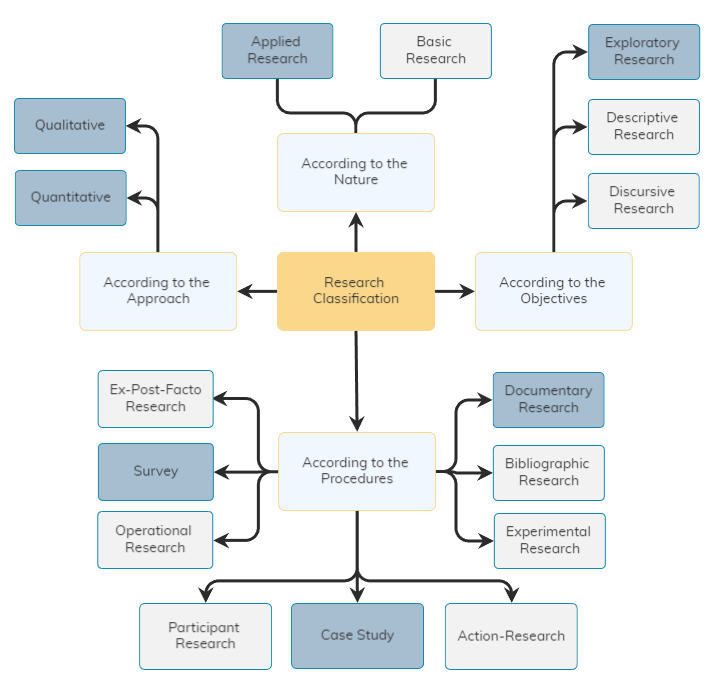
\includegraphics[width=0.70\textwidth]{imagens/2-pesquisa-survey.png}
% \end{figure}
\end{frame}
%######################################################################

%######################################################################
\begin{frame}{{\sffamily Desenho de Pesquisa}}
    \begin{figure}
    	\centering
    	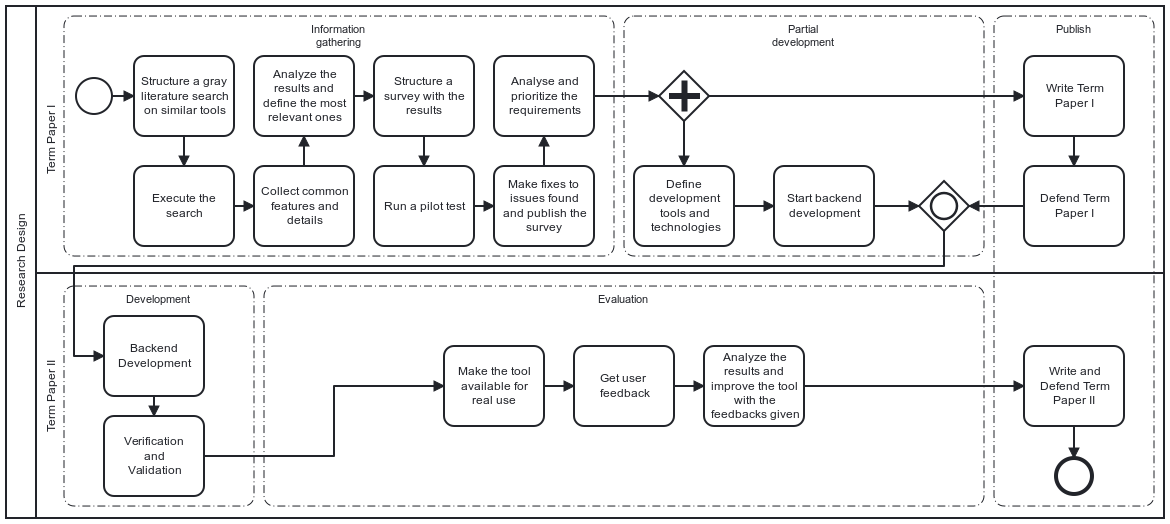
\includegraphics[width=1\textwidth, ]{imagens/2-research-diagram.png}
    \end{figure}
\end{frame}
%######################################################################

%######################################################################
\begin{frame}{{\sffamily Cronograma}}
\begin{table}[!htb]
  \centering
  \caption{Research Schedule}
  \label{tbl:schedule}
  \scriptsize
  \begin{tabular}{p{4cm}|l|lllll|lll}
    \bottomrule
    \rowcolor[rgb]{0.753,0.753,0.753} \multicolumn{1}{c|}{{\cellcolor[rgb]{0.753,0.753,0.753}}}                                       & \multicolumn{1}{c|}{\textbf{2021/2}} & \multicolumn{5}{c|}{\textbf{2022/1}} & \multicolumn{3}{c|}{\textbf{2022/2}}                                                                                                                                                                                                                                           \\
    \hhline{>{\arrayrulecolor[rgb]{0.753,0.753,0.753}}->{\arrayrulecolor{black}}---------|}
    \rowcolor[rgb]{0.753,0.753,0.753} \multicolumn{1}{c|}{\multirow{-2}{*}{{\cellcolor[rgb]{0.753,0.753,0.753}}\textbf{ Activities}}} & \textbf{Nov - Mar}                   & \multicolumn{1}{c}{\textbf{Apr}}     & \textbf{May}                         & \textbf{Jun}                         & \multicolumn{1}{l}{\textbf{Jul}}     & \textbf{Aug}                         & \textbf{Sep Oct Nov}                 & \textbf{Dec}                         & \multicolumn{1}{c|}{\textbf{Jan}}    \\
    \hline
    \rowcolor[rgb]{0.914,0.914,0.914} Plan and execute systematic review in the grey literature                                       & {\cellcolor[rgb]{0.753,0.753,0.753}} &                                      &                                      &                                      &                                      &                                      &                                      &                                      &                                      \\
    Plan and execute survey with target users                                                                                         &                                      & {\cellcolor[rgb]{0.753,0.753,0.753}} &                                      &                                      &                                      &                                      &                                      &                                      &                                      \\
    \rowcolor[rgb]{0.914,0.914,0.914} Analyze results from previous steps and map requirements                                        &                                      & {\cellcolor[rgb]{0.753,0.753,0.753}} & {\cellcolor[rgb]{0.753,0.753,0.753}} &                                      &                                      &                                      &                                      &                                      &                                      \\
    Plan and start tool development                                                                                                   &                                      &                                      & {\cellcolor[rgb]{0.753,0.753,0.753}} & {\cellcolor[rgb]{0.753,0.753,0.753}} &                                      &                                      &                                      &                                      &                                      \\
    \rowcolor[rgb]{0.914,0.914,0.914} Write Term Paper I                                                                              &                                      &                                      &                                      & {\cellcolor[rgb]{0.753,0.753,0.753}} & {\cellcolor[rgb]{0.753,0.753,0.753}} & {\cellcolor[rgb]{0.753,0.753,0.753}} &                                      &                                      &                                      \\
    Defend Term Paper I                                                                                                               &                                      &                                      &                                      &                                      &                                      & {\cellcolor[rgb]{0.753,0.753,0.753}} &                                      &                                      &                                      \\
    \rowcolor[rgb]{0.914,0.914,0.914} Continue the development of the tool                                                            &                                      &                                      &                                      &                                      &                                      & {\cellcolor[rgb]{0.753,0.753,0.753}} & {\cellcolor[rgb]{0.753,0.753,0.753}} & {\cellcolor[rgb]{0.753,0.753,0.753}} &                                      \\
    Execute a real use case on the tool                                                                                               &                                      &                                      &                                      &                                      &                                      &                                      &                                      & {\cellcolor[rgb]{0.753,0.753,0.753}} &                                      \\
    \rowcolor[rgb]{0.914,0.914,0.914} Write Term Paper II                                                                             &                                      &                                      &                                      &                                      &                                      &                                      &                                      & {\cellcolor[rgb]{0.753,0.753,0.753}} & {\cellcolor[rgb]{0.753,0.753,0.753}} \\
    Defend Term Paper II                                                                                                              &                                      &                                      &                                      &                                      &                                      &                                      &                                      &                                      & {\cellcolor[rgb]{0.753,0.753,0.753}} \\
    \toprule
  \end{tabular}
  \fonte{Author.}
\end{table}
\end{frame}
%######################################################################

%######################################################################
% \begin{frame}{{\sffamily Contexto de Pesquisa}}
% \begin{figure}
% 	\centering
% 	\caption{Contexto da Pesquisa: Solução de Teste de Desempenho}
% 	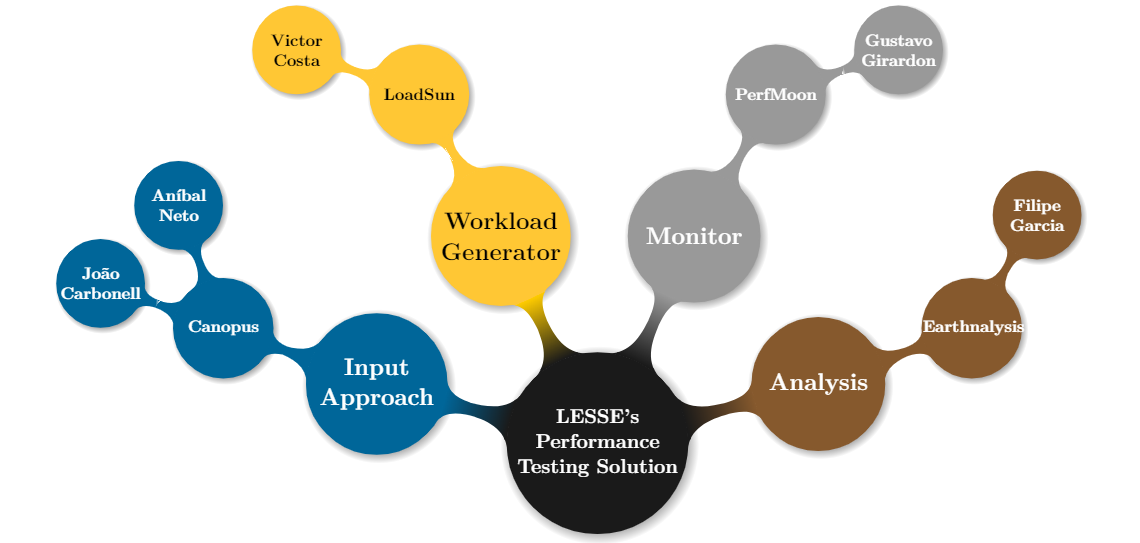
\includegraphics[width=0.89\textwidth]{Img/contexto.PNG}
% \end{figure}
% \end{frame}
%######################################################################

%######################################################################
% \begin{frame}{{\sffamily Síntese do Trabalho de Conclusão de Curso}}
% \begin{figure}
% 	\centering
% 	\caption{Síntese do Trabalho de Conclusão de Curso}
% 	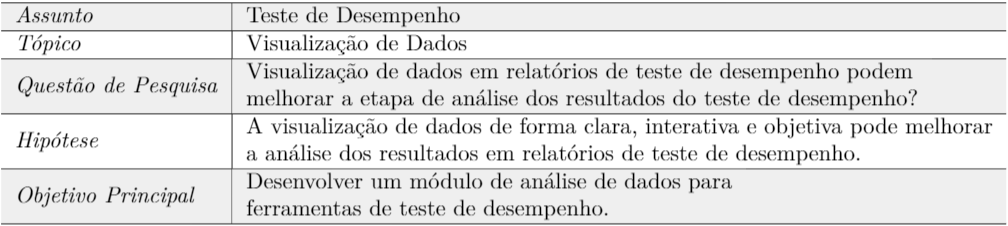
\includegraphics[width=0.99\textwidth]{Img/desenhodepesquisa.PNG}
% \end{figure}
% \end{frame}
%######################################################################

% \item Contexto
% 	        \SubItem{Curricularização da extensão}
% 	        \SubItem{Resoluções}
% 	        \SubItem{Unipampa Cidadã}
%---------------------------------------------------------------------
\section{Embasamento}
\subsection*{Embasamento}
%---------------------------------------------------------------------

%######################################################################
\begin{frame}{{\sffamily Curricularização da Extensão}}
\begin{block}{}
    \begin{itemize}
        \item Política Nacional de Extensão
            \SubItem{Extensão como solução para problemas sociais}
            \SubItem{Extensão como ferramenta essencial}
            \SubItem{Promover solidariedade e conscientização ambiental}
        \item Parte do curso como extensão (Res. 7 de 2018)
            \SubItem{10\% de horas do total}
            \SubItem{Adaptação em até 3 anos}
    \end{itemize}   


    % \begin{itemize}
    %     \item Parte do curso como extensão; %10% de horas, aumenta a procura e demanda
    %     \item Objetivos; %Garantir q extensão pode resolver qualquer problema social, promover solidariedade tanto nacional como internacionalmente, reconhecer que extensão é uma peça essencial em universidades publicas;
    %     \item Relação com a UNIPAMPA; %Teve que se adequar, ja vinha fazendo parte disso com RP por exemplo que gera a interação com publico de fora, comentar sobre experiencia gratificadora
    %     \item Documentos e processos de acordo com o definido. %Aumento de documentos necessarios pelo processo, autoavaliação ou a
    % \end{itemize}
\end{block}
\end{frame}
%######################################################################

%######################################################################
\begin{frame}{{\sffamily Curricularização da Extensão na UNIPAMPA}}
\begin{block}{}
    \begin{itemize}
        \item Disciplina de Resolução de Problemas
        \item Objetivos da Extensão pela (Res. 317 de 2021)
            \SubItem{Desenvolver a educação crítica, cívica, interdisciplinar e responsável}
            \SubItem{Fortalecer o vínculo entre ensino, pesquisa e extensão}
        \item Formalização pela (Res. 332 de 2021)
            \SubItem{Órgãos gestores, participantes da extensão, tramitações}% Quem coordena, quem participa, documentos necessarios, autoavaliação, minimo de duraç~ao de 8 horas
    \end{itemize}   

\end{block}
\end{frame}
%######################################################################

%######################################################################
\begin{frame}{{\sffamily Programas e Projetos de Extensão}}
% Objetivo não é criar um laço de dependência entre comunidades, so para resolver um determinado problema e deixar que eles consigam andar com as proprias pernas depois, por isso a qualidade
\begin{block}{O que são}
Ações que envolvem ensino, pesquisa e a comunidade externa.
\begin{itemize}
    \item Projetos possuem um objetivo específico e prazos determinados % Da pra falar das roles
    \item Um programa é um conjunto de projetos
\end{itemize}
\end{block}

\begin{block}{Exemplos de programas}
\begin{itemize}
    \item Programa C % Professora Aline
    \item Programa JEDI % Professor Bernardino
    \item Programa UniHacker.Club % Professor Diego
\end{itemize}
\end{block}

\end{frame}
%######################################################################

%######################################################################
% \begin{frame}{{\sffamily Resoluções}}
% \begin{block}{}
%     \begin{itemize}
%         \item a
%     \end{itemize}
% \end{block}
% \end{frame}
%######################################################################

%######################################################################
\begin{frame}{{\sffamily Unipampa Cidadã}}
\begin{block}{Unipampa Cidadã}
    \begin{itemize}
        \item Extensão curricular
        \item Atividades solidárias % Campanha do agasalho, 
            \SubItem{Campanha do agasalho, arrecadação de alimentos, suporte a asilos}
        \item Formação de egressos socialmente responsáveis % Egressos mais consientes com a responsabilidade social, Integração com a comunidade local
        \item Oferecida por todos os cursos 
            \SubItem{Mínimo de 60 e máximo de 120 horas}
        \item Formulário de finalização da atividade
    \end{itemize}
\end{block}
\end{frame}
%######################################################################

%---------------------------------------------------------------------

\section{Literatura Cinza}
\subsection*{Literatura Cinza}

%---------------------------------------------------------------------

%######################################################################
\begin{frame}{{\sffamily Literatura Cinza}}
\begin{block}{Motivação}
    \begin{itemize}
        \item Poucos resultados na literatura branca
        \item Na maioria das vezes ferramentas não possuem artigo publicado
    \end{itemize}
\end{block}

\begin{block}{Objetivos}
    \begin{itemize}
        \item Analisar ferramentas semelhantes ao MVP
            \SubItem{Funcionalidades e detalhes em comum}
        \item Extrair uma lista preliminar de requisitos
    \end{itemize}
\end{block}
Conduzido por dois alunos: Igor Costa e Lucas Fell.
\end{frame}
%######################################################################

%######################################################################
\begin{frame}{{\sffamily Questões de Pesquisa}}
    \begin{table}[!htb]
  \centering
  \label{tab:research-questions}
  \footnotesize
  \begin{tabular}{l|p{9cm}}
    \bottomrule
    \rowcolor[rgb]{0.753,0.753,0.753} \multicolumn{1}{c|}{\textbf{ID}} & \multicolumn{1}{c}{\textbf{Questão}}                                                                 \\
    \hline
    \rowcolor[rgb]{0.898,0.898,0.898} QP 1                            & Quais ferramentas existem atualmente que realizam gestão acadêmica?                                          \\
    QP 1.1                                                            & Quais delas possuem funcionalidades relacionadas ou dão suporte à atividades de extensão?                                 \\
    \rowcolor[rgb]{0.898,0.898,0.898} QP 1.2                          & Quais são as funcionalidades disponibilizadas por essas ferramentas?                                                         \\
    QP 1.3                                                            & Quais são as funcionalidades mais comuns entre este tipo de ferramenta?                                          \\
    \rowcolor[rgb]{0.898,0.898,0.898} QP 1.4                          & Quais dados as ferramentas usam em relação às atividades, cadastro de participantes e cadastro de usuários? \\
    \toprule
  \end{tabular}
\end{table}
\end{frame}
%######################################################################

%######################################################################
\begin{frame}{{\sffamily Critérios de Inclusão}}
\begin{block}{Duas etapas}
    \begin{enumerate}
        \item Diferenciação de ferramentas e catálogos
        \SubItem{Login, inscrição em atividades}
        \item Aplicação dos critérios de inclusão
    \end{enumerate}
\end{block}
        \begin{table}[!htb]
  \centering
%   \caption{Inclusion Criteria}
%   \label{tbl:gl-inclusion-criteria}
  \footnotesize
  \begin{tabular}{c|p{8cm}}
    \bottomrule
    \rowcolor[rgb]{0.753,0.753,0.753} \textbf{ID} & \multicolumn{1}{c}{\textbf{Critérios de Inclusão}}                     \\
    \hline
    \rowcolor[HTML]{DEDEDE}
    CI 1.                                         & A ferramenta ou site suporta o gerenciamento de atividades de extensão. \\
    CI 2.                                         & A ferramenta ou site tem uma versão estável.                           \\
    \rowcolor[HTML]{DEDEDE}
    CI 3.                                         & Se for uma ferramenta, deve ter documentação.                        \\
    \toprule
  \end{tabular}
%   \fonte{Author.}
\end{table}
\end{frame}
%######################################################################

%######################################################################
\begin{frame}{{\sffamily Critérios de Exclusão}}
    \begin{block}{Critérios de exclusão}
    Qualquer resultado que se encaixa em apenas um é automaticamente excluído.
\end{block}
        \begin{table}[!htb]
  \centering
%   \caption{Exclusion Criteria}
%   \label{tbl:gl-exclusion-criteria}
  \footnotesize
  \begin{tabular}{c|p{8cm}}
    \bottomrule
    \rowcolor[rgb]{0.753,0.753,0.753} \textbf{ID} & \multicolumn{1}{c}{\textbf{Critérios de Exclusão}}                                                           \\
    \hline
    \rowcolor[rgb]{0.898,0.898,0.898} CE 1.       & Se for uma ferramenta, não possui download do código-fonte ou página online.                               \\
    CE 2.                                         & A ferramenta ou o site não recebe atualizações há mais de 10 anos.                                  \\
    \rowcolor[rgb]{0.898,0.898,0.898} CE 3.       & A ferramenta ou site é de uso exclusivo da organização, ou seja, fechado ao público externo. \\
    CE 4.                                         & A ferramenta ou site é pago e não fornece uma versão de teste ou todas as atividades de extensão são pagas.     \\
    \toprule
  \end{tabular}
%   \fonte{Author.}
\end{table}
\end{frame}
%######################################################################

%######################################################################
\begin{frame}{{\sffamily Critérios de Qualidade}}
        \begin{block}{Atende ao critério?}
    Sim (1); Parcialmente (0.5); Não (0).
\end{block}
        \begin{table}[!htb]
  \centering
  \caption{Quality Criteria}
  \label{tbl:gl-quality-criteria}
  \arrayrulecolor{black}
  \footnotesize
  \begin{tabular}{c|p{4.2cm}|p{3cm}|p{2.5cm}|p{3cm}}
    \bottomrule
    \rowcolor[rgb]{0.753,0.753,0.753} {\cellcolor[rgb]{0.753,0.753,0.753}}                              & \multicolumn{1}{c|}{{\cellcolor[rgb]{0.753,0.753,0.753}}}                                            & \multicolumn{3}{c}{\textbf{\textbf{Score}}}                                                                                       \\
    \hhline{>{\arrayrulecolor[rgb]{0.753,0.753,0.753}}-->{\arrayrulecolor{black}}---}
    \rowcolor[rgb]{0.753,0.753,0.753} \multirow{-2}{*}{{\cellcolor[rgb]{0.753,0.753,0.753}}\textbf{ID}} & \multicolumn{1}{c|}{\multirow{-2}{*}{{\cellcolor[rgb]{0.753,0.753,0.753}}\textbf{Quality Criteria}}} & \multicolumn{1}{c|}{\textbf{Yes (1)}}       & \multicolumn{1}{c|}{\textbf{Partial (0.5)}} & \multicolumn{1}{c}{\textbf{No (0)}}   \\
    \hline
    \rowcolor[rgb]{0.898,0.898,0.898} QC 1.                                                             & Does the tool use a relevant amount of data related to outreach activities?                          & The tool uses >=20                          & 10 - 19                                     & 10 pieces of information              \\
    QC 2.                                                                                               & Does the tool have unique features among the selected tools?                                         & The tool has 1                              & 1                                           & No unique features                    \\
    \rowcolor[rgb]{0.898,0.898,0.898} QC 3.                                                             & Does the tool have a relevant amount of features among those collected?                              & The tool has >=14                           & 9-13                                        & 8 features in common with other tools \\
    \multicolumn{1}{l|}{QC 4.}                                                                          & Does the tool have specialized support?                                                              & Yes                                         & Partially                                   & No                                    \\
    \rowcolor[rgb]{0.898,0.898,0.898} \multicolumn{1}{l|}{QC 5.}                                        & Has the tool been maintained frequently?                                                             & The last update was in 2022                 & 2021-2019                                   & 2018 and before                       \\
    \toprule
  \end{tabular}
  \fonte{Author.}
\end{table}
\end{frame}
%######################################################################

%######################################################################
\begin{frame}{{\sffamily Condução}}
    % Divisão de trabalho
    % Período de tempo
    % Alteração nas strings
    \begin{block}{Divisão de trabalho}
    \begin{itemize}
        \item Dividido igualmente entre os dois autores
        \item Cada um analisou 500 resultados no total
    \end{itemize}
\end{block}
\begin{block}{Período de tempo}
Entre 17/02/2022 e 20/02/2022.
\end{block}
\begin{block}{Strings alteradas}
\begin{itemize}
    \item -SIGAA
    \item site:.edu.br
\end{itemize}
\end{block}
\end{frame}
%######################################################################

%######################################################################
\begin{frame}{{\sffamily Resultados}}
    % 169 encontradas e 12 depois 
    \begin{block}{Ferramentas encontradas}
        169 no total e 12 depois da aplicação dos critérios.
\end{block}
\begin{table}[!htb]
  \centering
  \caption{Search Results}
  \label{tbl:gl-search-results}
  \scriptsize
  \begin{tabular}{c|p{6cm}|l|p{1.5cm}|c}
    \bottomrule
    \rowcolor[rgb]{0.753,0.753,0.753} \textbf{No.} & \multicolumn{1}{c|}{\textbf{Search String}}                                                                                 & \textbf{Evaluated Results}  & \textcolor[rgb]{0.137,0.137,0.145}{\textbf{Potential New Tools}} & \textbf{Total} \\
    \hline
    \rowcolor[rgb]{0.898,0.898,0.898} 1            & sistema gestão acadêmicas (atividades \textbar{} projetos) site:.edu.br                                                     & 100 out of $\sim$1.250.000  & 4                                                                & 4              \\
    2                                              & (sistema \textbar{} ferramenta) gestão acadêmicas (atividades \textbar{} projetos) extensão site:.edu.br -SIGAA             & 100 out of $\sim$182.000    & 11                                                               & 15             \\
    \hhline{>{\arrayrulecolor[rgb]{0.898,0.898,0.898}}->{\arrayrulecolor{black}}->{\arrayrulecolor[rgb]{0.898,0.898,0.898}}---}
    \rowcolor[rgb]{0.898,0.898,0.898} 3            & (ferramenta \textbar{} aplicação) extensão (programa \textbar{} projeto) (gestão \textbar{} gerenciamento) -SIGAA           & 100 out of $\sim$15.600.000 & 9                                                                & 24             \\
    4                                              & (app \textbar{} aplicativo) extensão (programa \textbar{} projeto) (administração \textbar{} gerência) -SIGAA               & 100 out of $\sim$7.140.000  & 13                                                               & 37             \\
    \rowcolor[rgb]{0.898,0.898,0.898} 5            & ferramenta extensão (programa \textbar{} projeto) (gestão \textbar{} gerência) -SIGAA                                       & 100 out of $\sim$11.000.000 & 27                                                               & 64             \\
    6                                              & (ferramenta \textbar{} aplicação \textbar{} app \textbar{} aplicativo) extensão (programa \textbar{} projeto) gestão -SIGAA & 100 out of $\sim$22.500.000 & 15                                                               & 79             \\
    \rowcolor[rgb]{0.898,0.898,0.898} 7            & software extensão (programa \textbar{} projeto) (gerência \textbar{} gestão \textbar{} controle) -SIGAA                     & 100 out of $\sim$8.300.000  & 24                                                               & 103            \\
    8                                              & (software \textbar{} ferramenta \textbar{} aplicação) extensão atividade -SIGAA                                             & 100 out of $\sim$30.900.000 & 10                                                               & 113            \\
    \rowcolor[rgb]{0.898,0.898,0.898} 9            & sistema extensão (projeto \textbar{} programa \textbar{} atividade) gestão -SIGAA                                           & 100 out of $\sim$26.400.000 & 30                                                               & 143            \\
    10                                             & acadêmica extensão (projeto \textbar{} programa \textbar{} atividade) -SIGAA                                                & 100 out of $\sim$17.000.000 & 26                                                               & 169            \\
    \arrayrulecolor{black}\toprule
  \end{tabular}
  \fonte{Author.}
\end{table}
\end{frame}
%######################################################################

%######################################################################
\begin{frame}{{\sffamily Resultados}}
    % 37 funcionalidades algumas mescladas
    % SIGAA e CAEX mais pontuação
    \begin{block}{Funcionalidades encontradas}
    \begin{itemize}
        \item 37 no total, entre todas as ferramentas analisadas
        \item SIGAA e CAEX com a maior pontuação
    \end{itemize}
\end{block}
\begin{table}[!htb]
  \centering
  \caption{Quality Criteria Evaluation}
  \label{tbl:gl-quality-criteria-results}
  \arrayrulecolor{black}
  \scriptsize
  \begin{tabular}{c|p{2cm}|cc|cc|cc|cc|cc|c}
    \hhline{~~-----------}
    \multicolumn{2}{l}{\multirow{3}{*}{~ ~ ~ ~ ~ ~}}                                & \multicolumn{11}{c}{{\cellcolor[rgb]{0.753,0.753,0.753}}\textbf{Quality Criteria ~ ~ ~ ~ ~ ~ ~ ~}}                                                                                                                                                                                                                                                                                                                                                                                                                                                                                                                                                                                                                                                                                                                                                         \\
    \hhline{~~-----------}
    \multicolumn{2}{l}{}                                                            & \multicolumn{2}{c|}{{\cellcolor[rgb]{0.753,0.753,0.753}}\textbf{QC 1. ~}}                          & \multicolumn{2}{c|}{{\cellcolor[rgb]{0.753,0.753,0.753}}\textbf{QC 2. ~}} & \multicolumn{2}{c|}{{\cellcolor[rgb]{0.753,0.753,0.753}}\textbf{QC 3. ~}} & \multicolumn{2}{c|}{{\cellcolor[rgb]{0.753,0.753,0.753}}\textbf{QC 4. ~}} & \multicolumn{2}{c|}{{\cellcolor[rgb]{0.753,0.753,0.753}}\textbf{QC 5. }} & \multicolumn{1}{l}{{\cellcolor[rgb]{0.753,0.753,0.753}}}                                                                                                                                                                                                                                                                                                                                                                               \\
    \multicolumn{2}{l}{}                                                            & {\cellcolor[rgb]{0.753,0.753,0.753}}\textbf{Ans.}                                                  & {\cellcolor[rgb]{0.753,0.753,0.753}}\textbf{Score}                        & {\cellcolor[rgb]{0.753,0.753,0.753}}\textbf{Ans.}                         & {\cellcolor[rgb]{0.753,0.753,0.753}}\textbf{Score}                        & {\cellcolor[rgb]{0.753,0.753,0.753}}\textbf{Ans.}                        & {\cellcolor[rgb]{0.753,0.753,0.753}}\textbf{Score}       & {\cellcolor[rgb]{0.753,0.753,0.753}}\textbf{Ans.} & {\cellcolor[rgb]{0.753,0.753,0.753}}\textbf{Score} & {\cellcolor[rgb]{0.753,0.753,0.753}}\textbf{Ans.} & {\cellcolor[rgb]{0.753,0.753,0.753}}\textbf{Score} & \multicolumn{1}{l}{\multirow{-2}{*}{{\cellcolor[rgb]{0.753,0.753,0.753}}\begin{tabular}[c]{@{}l@{}}\textbf{Final}\\\textbf{Results }\end{tabular}}}       \\
    \hhline{>{\arrayrulecolor[rgb]{0.753,0.753,0.753}}-->{\arrayrulecolor{black}}-----------}
    \rowcolor[rgb]{0.898,0.898,0.898} {\cellcolor[rgb]{0.753,0.753,0.753}}          & {\cellcolor[rgb]{0.753,0.753,0.753}}\textbf{Cachalote}                                             & 9                                                                         & 0,0                                                                       & No                                                                        & 0,0                                                                      & 12                                                       & 0,5                                               & Partially                                          & 0,5                                               & 2021                                               & 0,5                                                                                                                                                 & 1,5 \\
    {\cellcolor[rgb]{0.753,0.753,0.753}}                                            & {\cellcolor[rgb]{0.753,0.753,0.753}}\textbf{CAEX}                                                  & 4                                                                         & 0,0                                                                       & 7                                                                         & 1,0                                                                      & 22                                                       & 1,0                                               & Yes                                                & 1,0                                               & 2022                                               & 1,0                                                                                                                                                 & 4,0 \\
    \rowcolor[rgb]{0.898,0.898,0.898} {\cellcolor[rgb]{0.753,0.753,0.753}}          & {\cellcolor[rgb]{0.753,0.753,0.753}}\textbf{Einstein}                                              & 12                                                                        & 0,5                                                                       & 1                                                                         & 0,5                                                                      & 13                                                       & 0,5                                               & Partially                                          & 0,5                                               & 2022                                               & 1,0                                                                                                                                                 & 3,0 \\
    {\cellcolor[rgb]{0.753,0.753,0.753}}                                            & {\cellcolor[rgb]{0.753,0.753,0.753}}\textbf{ENS}                                                   & 11                                                                        & 0,5                                                                       & 3                                                                         & 1,0                                                                      & 12                                                       & 0,5                                               & Partially                                          & 0,5                                               & 2022                                               & 1,0                                                                                                                                                 & 3,5 \\
    \rowcolor[rgb]{0.898,0.898,0.898} {\cellcolor[rgb]{0.753,0.753,0.753}}          & {\cellcolor[rgb]{0.753,0.753,0.753}}\textbf{Santa Marcelina}                                       & 6                                                                         & 0,0                                                                       & No                                                                        & 0,0                                                                      & 7                                                        & 0,0                                               & Partially                                          & 0,5                                               & 2022                                               & 1,0                                                                                                                                                 & 1,5 \\
    {\cellcolor[rgb]{0.753,0.753,0.753}}                                            & {\cellcolor[rgb]{0.753,0.753,0.753}}\textbf{SGE}                                                   & 8                                                                         & 0,0                                                                       & 1                                                                         & 0,5                                                                      & 14                                                       & 1,0                                               & Yes                                                & 1,0                                               & 2016                                               & 0,0                                                                                                                                                 & 2,5 \\
    \rowcolor[rgb]{0.898,0.898,0.898} {\cellcolor[rgb]{0.753,0.753,0.753}}          & {\cellcolor[rgb]{0.753,0.753,0.753}}\textbf{SIEX}                                                  & 53                                                                        & 1,0                                                                       & 1                                                                         & 0,5                                                                      & 7                                                        & 0,0                                               & Yes                                                & 1,0                                               & 2022                                               & 1,0                                                                                                                                                 & 3,5 \\
    {\cellcolor[rgb]{0.753,0.753,0.753}}                                            & {\cellcolor[rgb]{0.753,0.753,0.753}}\textbf{SIG}                                                   & 18                                                                        & 0,5                                                                       & No                                                                        & 0,0                                                                      & 15                                                       & 1,0                                               & Partially                                          & 0,5                                               & 2022                                               & 1,0                                                                                                                                                 & 3,0 \\
    \rowcolor[rgb]{0.898,0.898,0.898} {\cellcolor[rgb]{0.753,0.753,0.753}}          & {\cellcolor[rgb]{0.753,0.753,0.753}}\textbf{SIGAA}                                                 & 28                                                                        & 1,0                                                                       & 1                                                                         & 0,5                                                                      & 16                                                       & 1,0                                               & Yes                                                & 1,0                                               & 2022                                               & 1,0                                                                                                                                                 & 4,5 \\
    {\cellcolor[rgb]{0.753,0.753,0.753}}                                            & {\cellcolor[rgb]{0.753,0.753,0.753}}\textbf{Suap}                                                  & 8                                                                         & 0,0                                                                       & No                                                                        & 0,0                                                                      & 10                                                       & 0,5                                               & Yes                                                & 1,0                                               & 2022                                               & 1,0                                                                                                                                                 & 2,5 \\
    \rowcolor[rgb]{0.898,0.898,0.898} {\cellcolor[rgb]{0.753,0.753,0.753}}          & {\cellcolor[rgb]{0.753,0.753,0.753}}\textbf{UNINASSAU}                                             & 14                                                                        & 0,5                                                                       & No                                                                        & 0,0                                                                      & 10                                                       & 0,5                                               & Partially                                          & 0,5                                               & 2022                                               & 1,0                                                                                                                                                 & 2,5 \\
    \multirow{-12}{*}{{\cellcolor[rgb]{0.753,0.753,0.753}}\rotcell{\textbf{Tools}}} & {\cellcolor[rgb]{0.753,0.753,0.753}}\textbf{UNINTER}                                               & 9                                                                         & 0,0                                                                       & No                                                                        & 0,0                                                                      & 13                                                       & 0,5                                               & Partially                                          & 0,5                                               & 2022                                               & 1,0                                                                                                                                                 & 2,0 \\
    \toprule
  \end{tabular}

  \fonte{Author.}
\end{table}
    
    % Respostas as questões de pesquisa
    % Ajuda 
    % (QP1) Resultados que passaram no CI1.
    % (QP1.1, QP1.2, QP1.3) Matriz de funcionalidades
    % (QP1.4) Segunda extração de dados
\end{frame}
%######################################################################
\section{Survey}
\subsection*{Survey}

\begin{frame}{{\sffamily Levantamento (Survey)}}
  \begin{block}{Por que um levantamento?}
    \begin{itemize}
      \item Generalizar sobre as crenças e opiniões de muitas pessoas estudando apenas um subconjunto delas.
    \end{itemize}
  \end{block}
  \begin{block}{Objetivo}
    \begin{itemize}
      \item Entender as necessidades de alunos e professores em relação a projetos e atividades de extensão.
    \end{itemize}
  \end{block}
  Conduzido por dois alunos: Igor Costa e Lucas Fell.
\end{frame}

\begin{frame}{{\sffamily Objetivos e Estrutura}}
  \begin{block}{Objetivo de pesquisa}
    \begin{itemize}
      \item Ordenar e refinar os requisitos elicitados na revisão sistemática
    \end{itemize}
  \end{block}
  \begin{block}{Estrutura do questionário}
    \begin{itemize}
      \item Histórias de usuário
            \SubItem{Ranqueamento MoSCoW adaptado (InIDeIr)}
      \item Sugestões livres mais elaboradas
    \end{itemize}
  \end{block}
\end{frame}

\begin{frame}{{\sffamily Identificação e Questões}}
  \begin{block}{Identificação}
    \begin{itemize}
      \item Público alvo
            \SubItem{Comunidade acadêmica}
      \item Dados de identificação
            \SubItem{Gênero, educação, faixa etária, papel na extensão}
      \item Separação da amostra
            \SubItem{Discentes, Docentes e TAEs}
    \end{itemize}
  \end{block}
\end{frame}

\begin{frame}{{\sffamily Identificação e Questões}}
  \begin{block}{Questões}
    \begin{itemize}
      \item Discentes: 14 questões
      \item Docentes/TAEs: 11 questões
    \end{itemize}
  \end{block}
\end{frame}


\begin{frame}{{\sffamily Identificação e Questões}}

\begin{columns}
\begin{column}{0.5\textwidth}
   \begin{figure}
        \centering
        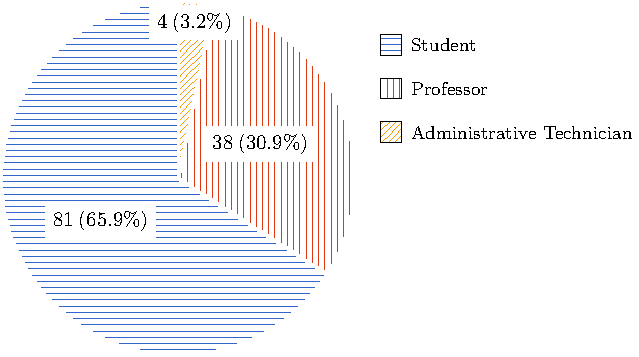
\includegraphics[width=6cm, ]{imagens/5-community-roles.pdf}
    \end{figure}
\end{column}
\begin{column}{0.5\textwidth}  %%<--- here
\begin{figure}
        \centering
        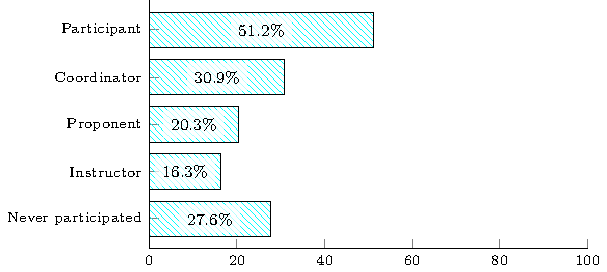
\includegraphics[width=5.5cm, ]{imagens/5-outreach-roles.pdf}
    \end{figure}
    % \begin{center}
    %  \includegraphics[width=0.5\textwidth]{image1.jpg}
    %  \end{center}
\end{column}
\end{columns}
\end{frame}


% \begin{frame}{{\sffamily Identificação e Questões}}
%   \
% \end{frame}

\begin{frame}{{\sffamily Resultados}}
  \begin{block}{Resultados}
    \begin{itemize}
      \item 123 respostas no total
      \item 23\% e 12\% de respostas qualitativas para professores e alunos, respectivamente
    \end{itemize}
  \end{block}
\end{frame}

\begin{frame}{{\sffamily Resultados - Análise quantitativa}}
  \begin{block}{Questão 1 dos docentes/TAEs}
    ``P1 - Eu como Proponente, gostaria de propor uma atividade de extensão, criando oportunidades de conhecimento para outras pessoas.''
  \end{block}
\end{frame}

\begin{frame}{{\sffamily Resultados - Análise quantitativa}}
  \begin{figure}
    \centering
    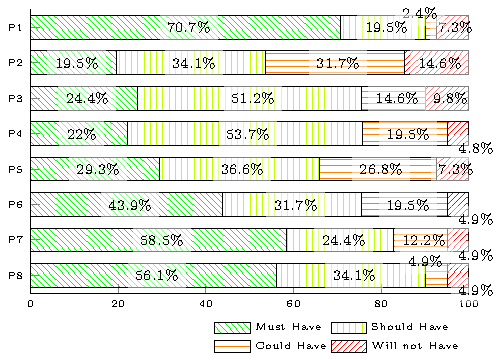
\includegraphics[width=8cm, ]{imagens/5-questions-proponent.pdf}
  \end{figure}
\end{frame}

\begin{frame}{{\sffamily Resultados - Análise quantitativa}}
  \begin{block}{Questão 11 dos alunos}
    ``A11 - Eu como Participante, gostaria de realizar a inscrição em atividades de extensão sem fazer cadastro no sistema, para que minhas informações não sejam salvas.''
  \end{block}
\end{frame}

\begin{frame}{{\sffamily Resultados - Análise quantitativa}}
  \begin{figure}
    \centering
    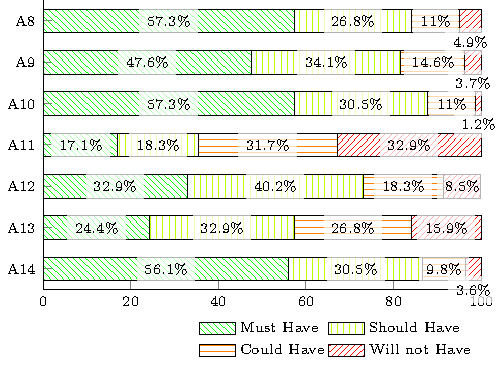
\includegraphics[width=8cm, ]{imagens/5-questions-participant-2.pdf}
  \end{figure}
\end{frame}

\begin{frame}{{\sffamily Resultados - Análise qualitativa}}
  Novos requisitos levantados baseado nas sugestões:
  \begin{block}{Professores/TAEs}
    \begin{itemize}
      \item Geração de certificados em conjunto
      \item Geração de relatórios no formato do programa SAP
      \item Priorização de participantes
      \item Certificado de inscrição
    \end{itemize}
  \end{block}
  \begin{block}{Alunos}
    \begin{itemize}
      \item Notificações (prazo de inscrição)
    \end{itemize}
  \end{block}
\end{frame}

\begin{frame}{{\sffamily Ameaças à validade}}
  \begin{block}{Ameaças à validade}
    \begin{itemize}
      \item Escala MoSCoW
            \SubItem{Engenharia de Software}
      \item Histórias de usuário muito descritas
            \SubItem{Difícil de encontrar novas funcionalidades}
      \item Falta de clareza nos termos
    \end{itemize}
  \end{block}
\end{frame}

%---------------------------------------------------------------------

\section{MVP}
\subsection*{MVP}

%---------------------------------------------------------------------
% \SubItem{Perfis de Usuário}
% 	        \SubItem{Arquitetura}
% 	        \SubItem{Licença}
% 	        \SubItem{DevOps}
%######################################################################
\begin{frame}{{\sffamily Análise e Projeto do MVP}}
\begin{block}{Perfis de Usuário}
    \begin{itemize}
        \item Participante
        \item Instrutor
        \item Proponente
        \item Coordenador
        \item Supervisor
        
        \item Participante Externo
    \end{itemize}
\end{block}
\end{frame}
%######################################################################}

%######################################################################
\begin{frame}{{\sffamily Casos de Uso}}
    \begin{figure}
        \vfill
        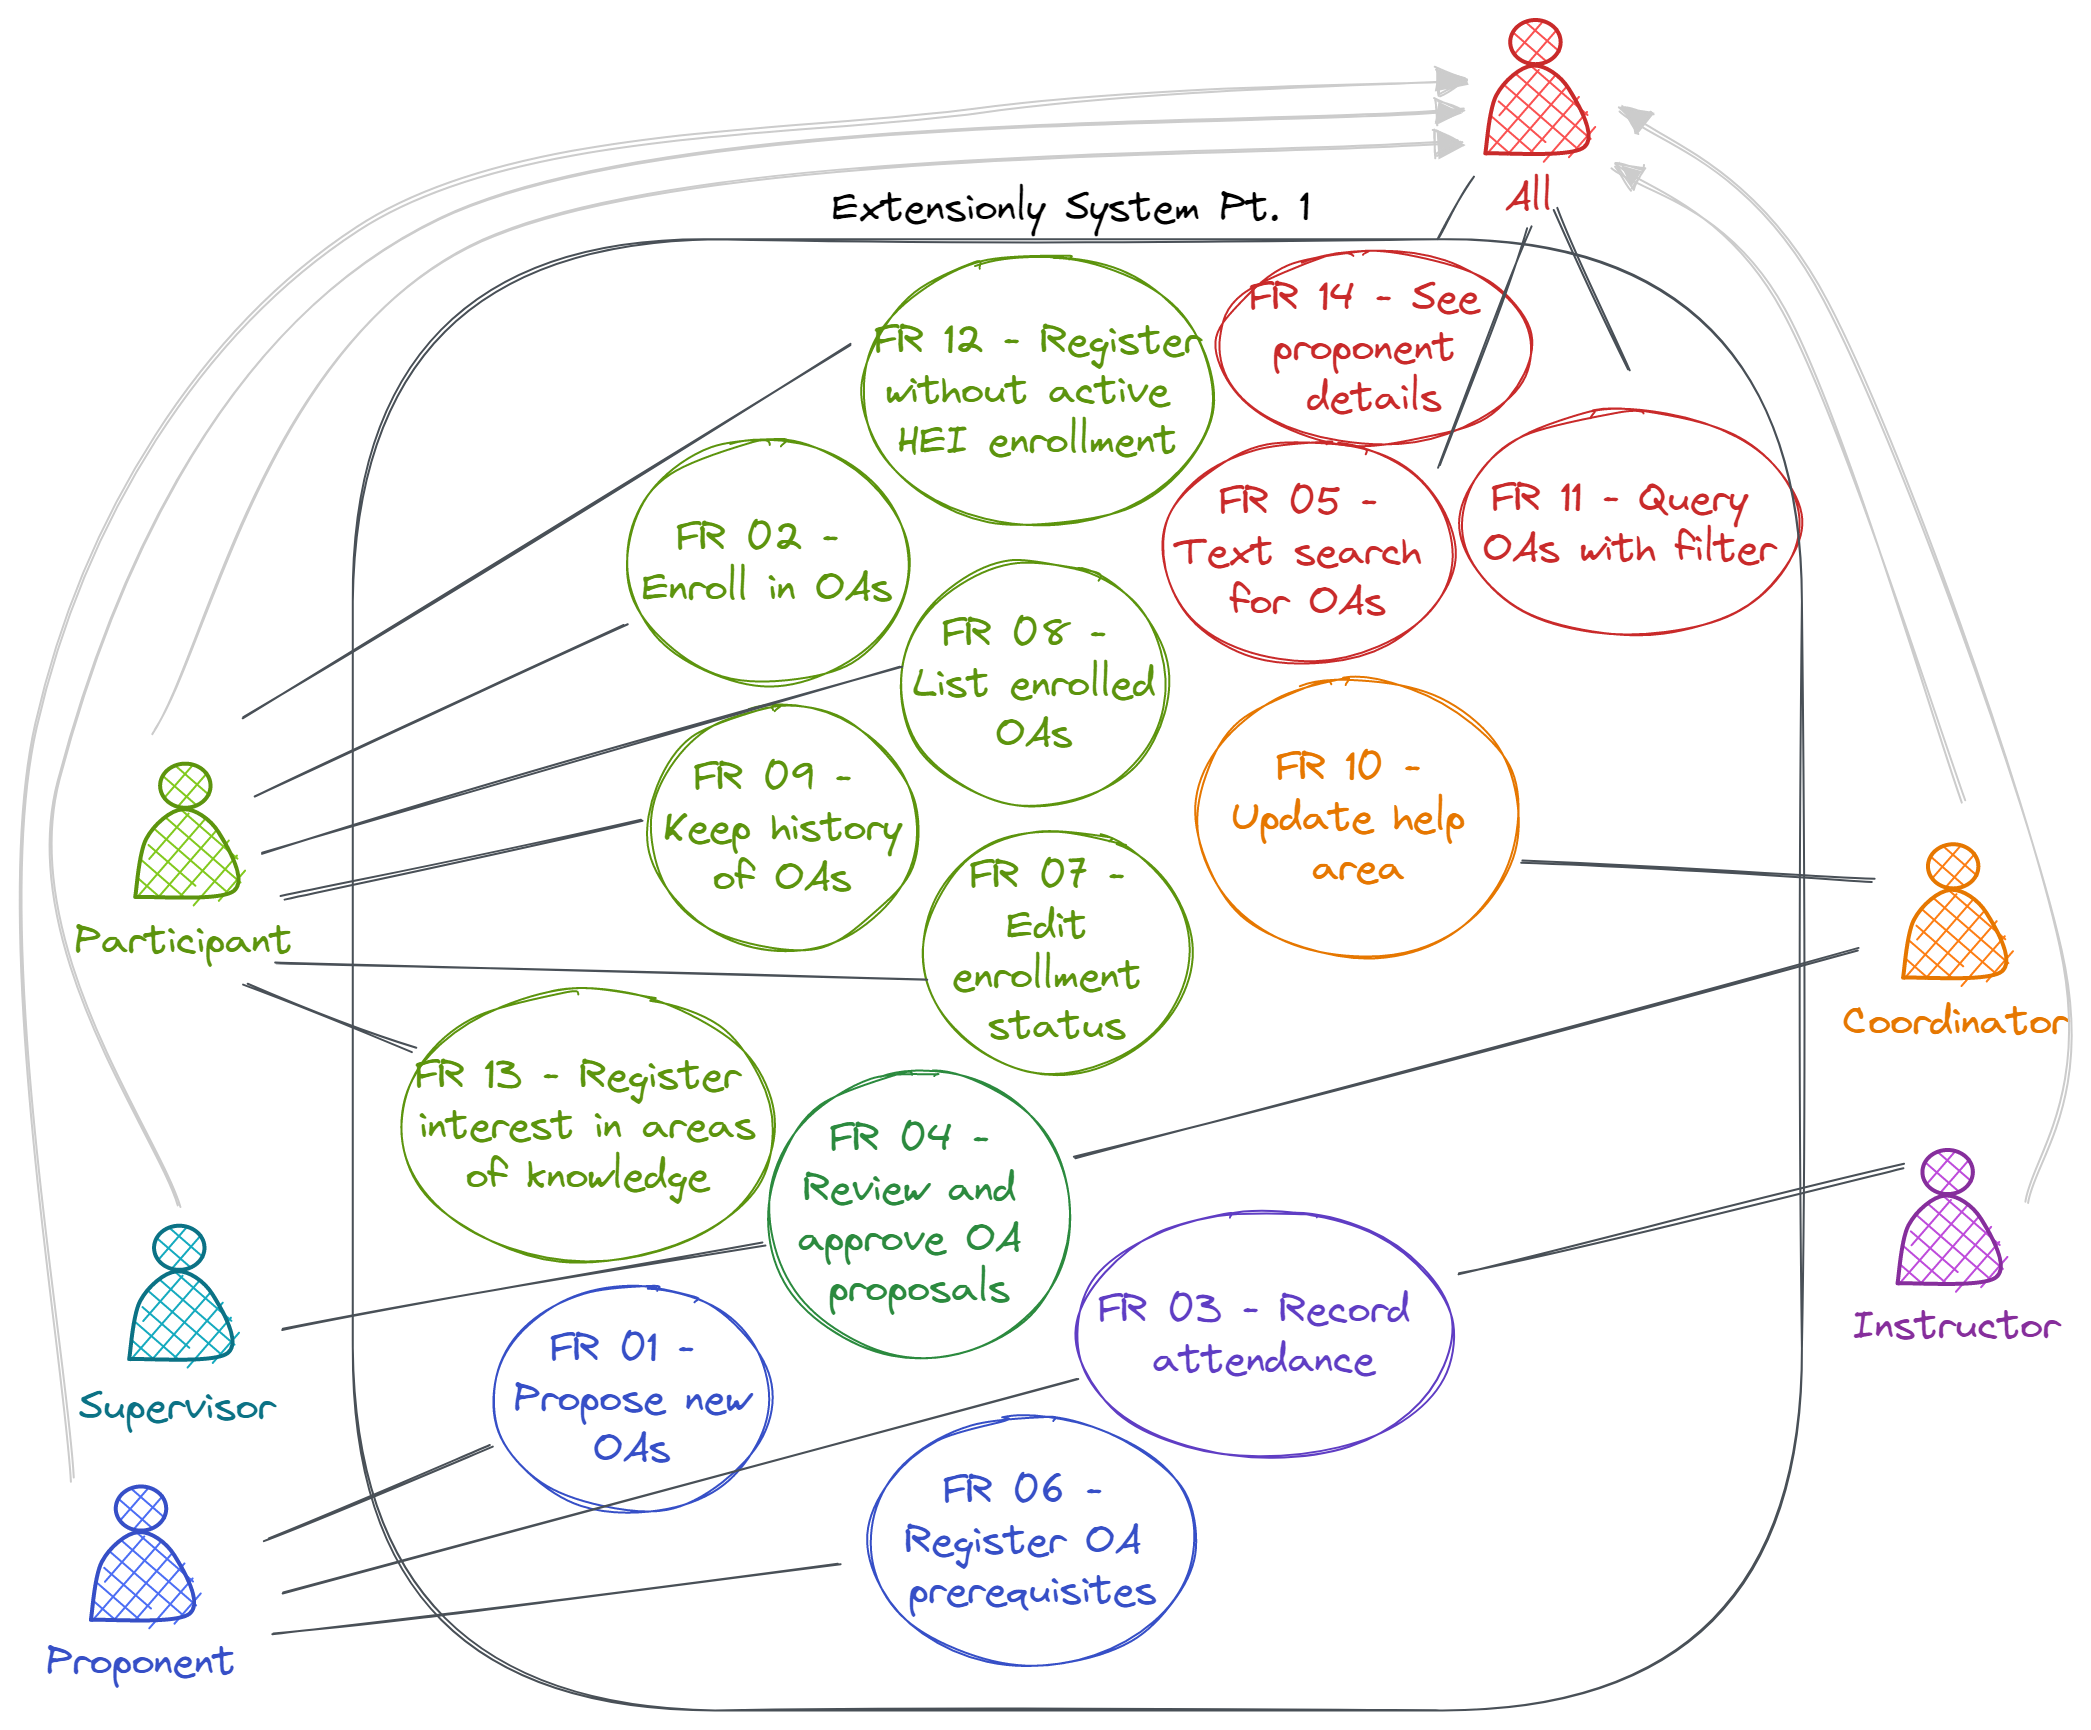
\includegraphics[width=7.5cm, ]{imagens/6-use-case-1.png}
        \vfill
    \end{figure}
\end{frame}
%######################################################################}

%######################################################################
\begin{frame}{{\sffamily Casos de Uso}}
    \begin{figure}
        \vfill
        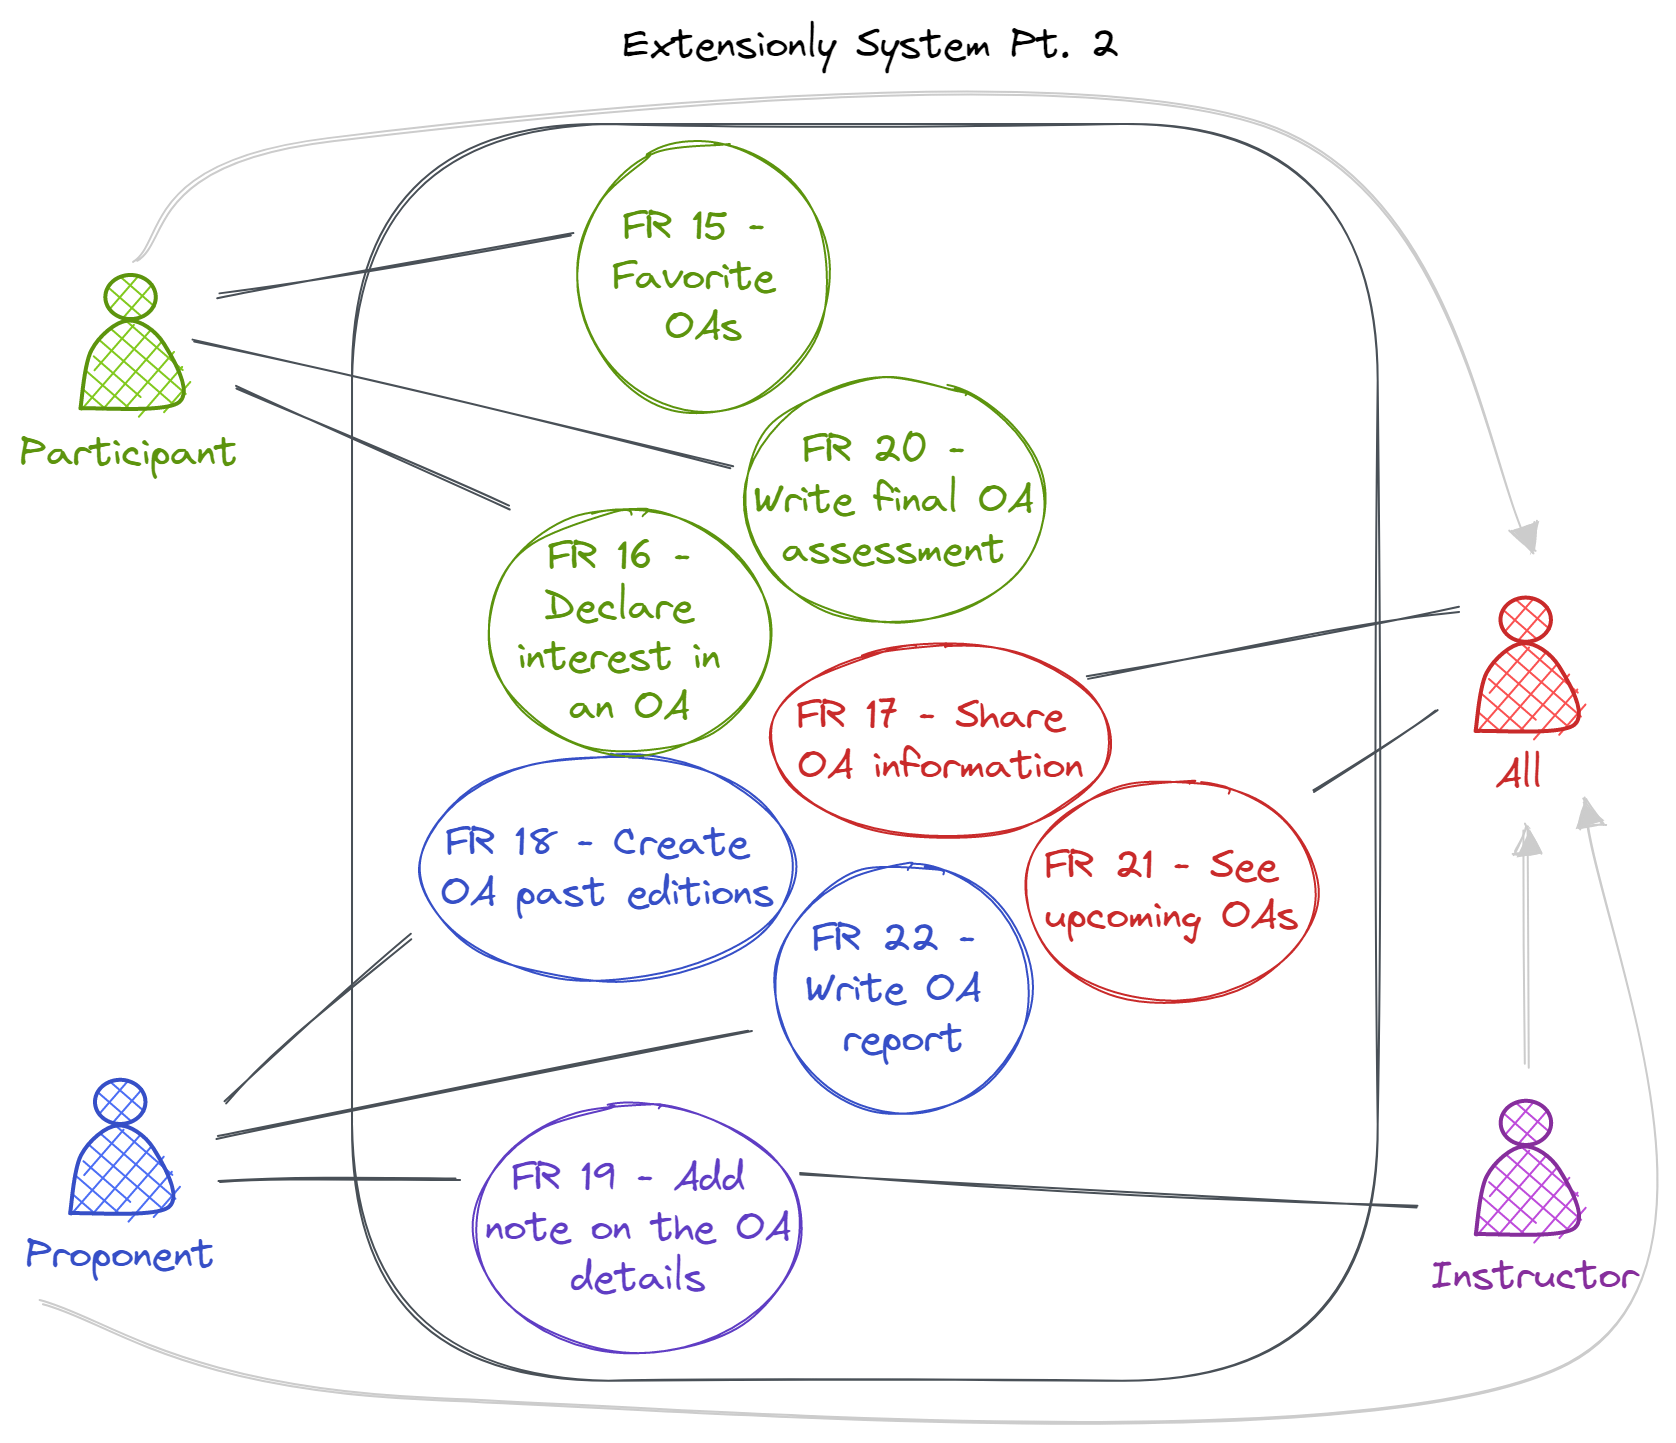
\includegraphics[width=7.5cm, ]{imagens/6-use-case-2.png}
        \vfill
    \end{figure}
\end{frame}
%######################################################################}

%######################################################################
\begin{frame}{{\sffamily Análise e Projeto do MVP}}
\begin{block}{Decisões de Projeto}
    \begin{itemize}
        \item Linguagem de programação: 
            \SubItem{TypeScript}
        \item Framework: 
            \SubItem{NestJs}
        \item Arquitetura: 
            \SubItem{Cliente-Servidor}
        \item Persistência de dados:
            \SubItem{MySQL}
            \SubItem{Prisma (ORM)}
    \end{itemize}
\end{block}
\end{frame}
%######################################################################}

%######################################################################
\begin{frame}{{\sffamily Arquitetura}}
% % \frame[allowpagebreak,T]
% % {%
%         \only<1>
%         {%
%             \centering
%             \vfill
%             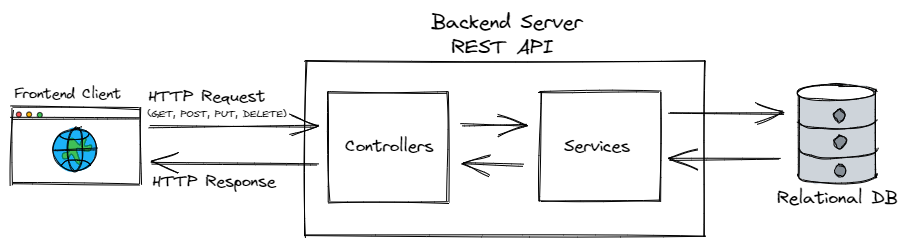
\includegraphics[height=2cm\textheight-0.5in]{imagens/6-architecture.png}
%         }%
% % }
    \begin{figure}
        \vfill
        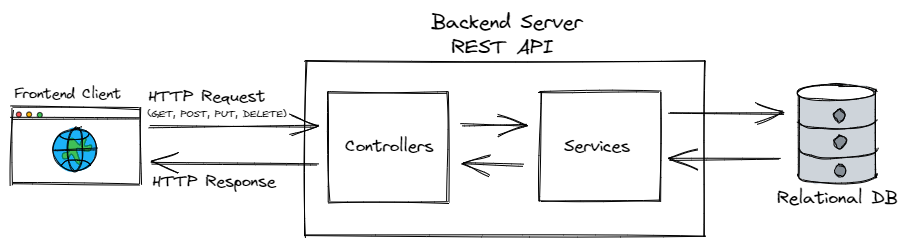
\includegraphics[width=10.5cm, ]{imagens/6-architecture.png}
        \vfill
    \end{figure}

\end{frame}
%######################################################################}

%######################################################################
\begin{frame}{{\sffamily DevOps}}
\begin{block}{DevOps}
    \begin{itemize}
        \item Integração Contínua (CI):
            \SubItem{Divisão de branches}
            \SubItem{Pipelines para testes automatizados}
        \item Entrega Contínua (CDE):
            \SubItem{Versionamento por tags}
            \SubItem{Pipelines para deploy}
        \item Solução PaaS do Heroku
    \end{itemize}
\end{block}
\end{frame}
%######################################################################}

%---------------------------------------------------------------------

\section{Conclusão}
\subsection*{Conclusão}

%---------------------------------------------------------------------

%######################################################################
\begin{frame}{{\sffamily Conclusões Preliminares}}
\begin{block}{Objetivos atingidos}
    \begin{itemize}
        \item Revisão da literatura cinza para procurar funcionalidades em ferramentas semelhantes
        \item Levantamento para entender os pontos de vista de usuários finais
        \item Pesquisar, avaliar e selecionar tecnologias para o MVP
    \end{itemize}
\end{block}
\begin{block}{Objetivos parciais}
    \begin{itemize}
        \item Roadmap de implementação e tarefas tangíveis
        \SubItem{TCC II}
    \end{itemize}
\end{block}
\end{frame}
\begin{frame}{{\sffamily Conclusões Preliminares}}
\begin{block}{Objetivos não atingidos}
    \begin{itemize}
        \item Desenvolvimento do MVP
        \SubItem{TCC II}
    \end{itemize}
\end{block}
\end{frame}
%######################################################################}

%######################################################################
% \begin{frame}{{\sffamily  Revisão Sistemática}}
%     \begin{figure}
%         \centering
%         \caption{Processo de Revisão Sistemática de Literatura (NAKAGAWA, E. et al.)} 
%         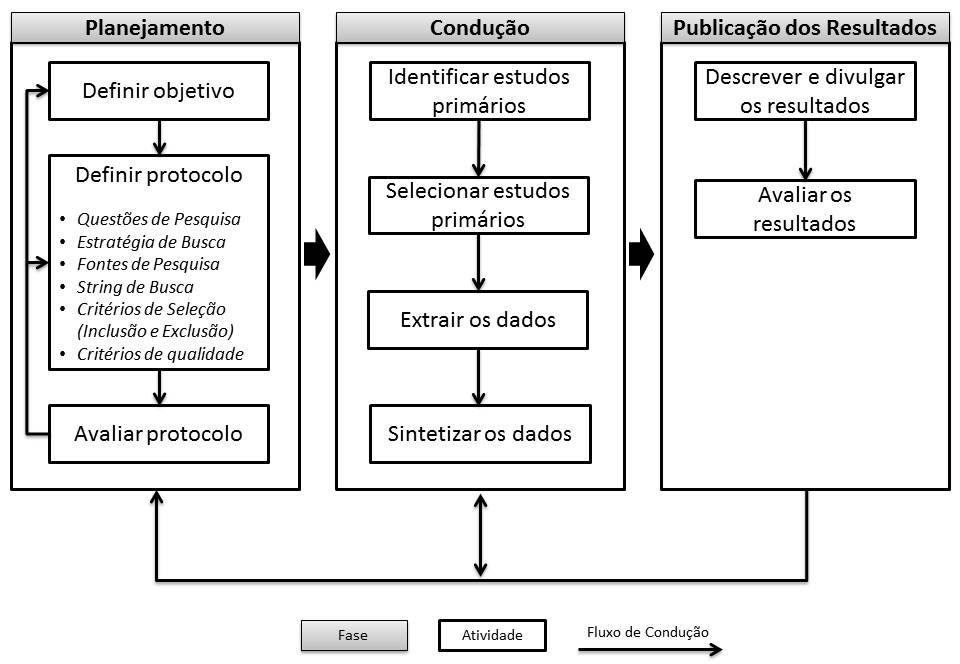
\includegraphics[width=0.68\textwidth]{Img/ProtocoloRS2.jpg}
%     \end{figure}
% \end{frame}
%######################################################################

% \begin{frame}{{\sffamily  Revisão Sistemática: Critérios de Inclusão}}
% \begin{block}{}
% 	\begin{itemize}%[<+->]
% 	        \item{CI1.O estudo deve citar uma ferramenta de teste de desempenho;}
% 	        \item{CI2.O estudo deve possuir avaliação empírica e expositiva sobre a ferramenta abordada;}
% 	        \item{CI3.Métricas e/ou padrões/normas de qualidade que apoiam a avaliação de uma ferramenta de teste de desempenho;}
% 	\end{itemize}
% \end{block}
% \end{frame}

% \begin{frame}{{\sffamily  Revisão Sistemática: Critérios de Exclusão}}
% \begin{block}{}
% 	\begin{itemize}%[<+->]
% 	        \item{CE1.Estudos duplicados;}
% 	        \item{CE2.O estudo não está escrito em inglês;}
% 	        \item{CE3.O estudo não fornece acesso completo ao seu conteúdo;}
% 	        \item{CE4.O estudo possui menos de 6 páginas, i.e., resumos expandidos;}
% 	\end{itemize}
% \end{block}
% \end{frame}

% \begin{frame}{{\sffamily  Revisão Sistemática: Goal Questions and Metrics}}
%     \begin{figure}
%         \centering
%         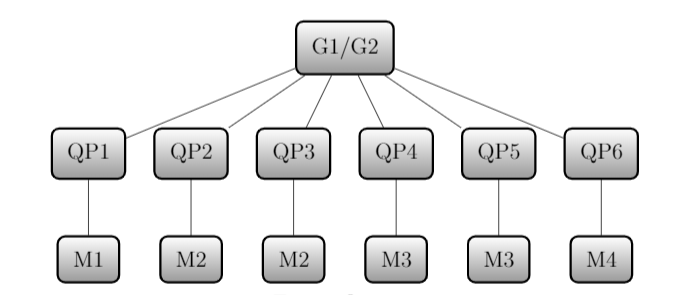
\includegraphics[width=0.95\textwidth]{Img/gqm.png}
%     \end{figure}
% \end{frame}

% \begin{frame}{{\sffamily  Revisão Sistemática: Questões de Pesquisa}}
% \begin{block}{}
% 	\begin{itemize}%[<+->]
% 	        \item{G1.Identificar quais são as ferramentas de teste de desempenho, e mapear suas funcionalidades.}
% 	        \SubItem{QP1.Quais são as ferramentas que apoiam o teste de desempenho?}
% 	        \SubItem{QP2.Quais as funcionalidades das ferramentas de teste de desempenho?}
% 	        \SubItem{QP3.Quais as abordagens de integração entre os artefatos de teste gerados nas ferra-mentas de teste de desempenho?}
% 	 \end{itemize}
% \end{block}
% \end{frame}

% \begin{frame}{{\sffamily  Revisão Sistemática: Questões de Pesquisa}}
% \begin{block}{}
% 	\begin{itemize}%[<+->]
% 	        \item{G2.Identificar abordagens, bibliotecas e ferramentas para visualização de dados,as quais possam ser utilizadas na análise de dados em relatórios de teste de desempenho.}
% 	        \SubItem{QP4.Quais as abordagens de apresentação dos resultados do teste de desempenho?}
% 	        \SubItem{QP5.Quais as abordagens de análise de resultados do teste de desempenho?}
% 	        \SubItem{QP6.Quais são as bibliotecas e ferramentas de visualização de dados a partir de uma entrada de dados?}
% 	 \end{itemize}
% \end{block}
% \end{frame}

% \begin{frame}{{\sffamily  Revisão Sistemática: Métricas}}
% \begin{block}{}
% 	\begin{itemize}%[<+->]
% 	        \item{M1.Nomes das ferramentas de teste de desempenho encontradas no estudo;}
% 	        \item{M2.Quais as funcionalidades das ferramentas;}
% 	        \item{M3.Abordagem de apresentação dos dados;}
% 	        \item{M4.Bibliotecas e ferramentas de visualização de dados.}
%     \end{itemize}
% \end{block}
% \end{frame}


% \begin{frame}{{\sffamily  Revisão Sistemática: String de Busca}}
    
% \begin{table}[!h]
% \centering
% \footnotesize
% \label{tab:DefinicaoSearch}
% \begin{tabular}{m{3cm}|m{6cm}}
% \bottomrule
% \rowcolor[HTML]{C0C0C0}
% \textbf{Termos} & \textbf{Sinônimos}
%  \\
% %\midrule 
% \rowcolor[HTML]{EFEFEF}
% \hline
% {\textbf{Performance Test}} & Load test, Stress test, Spike test, Workload test, Automation test 
%  \\
% %\midrule
% \hline
% \textbf{Tool} & Monitor, Generator, Plugin, Plug-in, Framework, Injector, Suite, Analyzer, Environment
% \\
% %\midrule
% \hline
% \toprule
% \end{tabular}
% \end{table}


% \begin{figure}[htb]
% \centering
% \fbox{\
% \normalsize
% \parbox{10cm}{
% \centering
% \scriptsize\texttt{
% (Performance test OR Load test OR Stress test OR Spike test OR Soak test OR Workload test OR Automation test) AND (Tool OR Monitor OR Generator OR Plugin OR Plug-in OR Framework OR Injector OR Suite OR Environment) AND (Software OR Application OR System)}}}
% \label{fig:StringBusca}
% \end{figure}

% \end{frame}

% \begin{frame}{{\sffamily  Revisão Sistemática: Estudos Primários}}
%     \begin{figure}[!h]
% 	\centering
% 	\caption{Estudos primários retornados nas bases de dados} 
% 		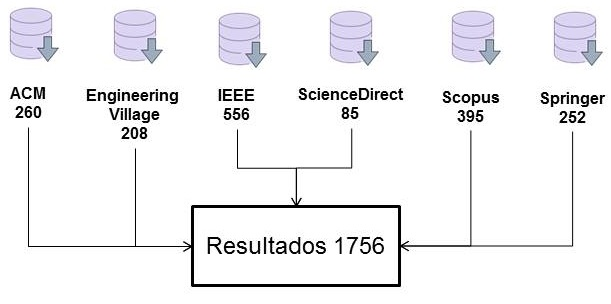
\includegraphics[width=.70\textwidth]{Img/ResultadosBases.JPG}
% 	\label{fig:ResusltadosBases}
% \end{figure}
%  \end{frame}

% % \begin{frame}{{\sffamily  Revisão Sistemática: Resultados dos Estudos Primários}}
% %     \begin{figure}
% %         \centering
% %         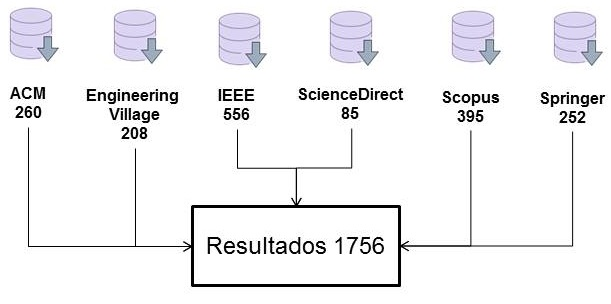
\includegraphics[width=0.99\textwidth]{Img/ResultadosBases.JPG}
% %         \end{figure}
% % \end{frame}

% \begin{frame}{{\sffamily  Revisão Sistemática: Processo de Seleção dos Estudos. }}
% \begin{figure}
%     \centering
%     \caption{Processo de Seleção dos Estudos.}
%     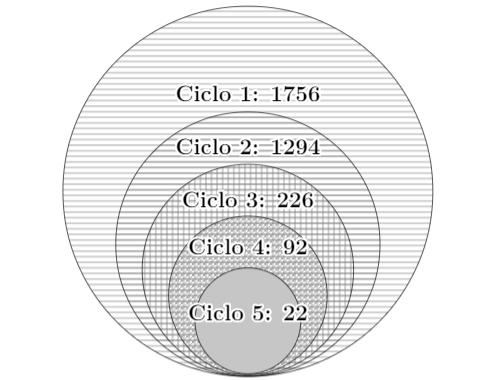
\includegraphics[width=0.70\textwidth]{Img/ciclos.PNG}
% \end{figure}
% \end{frame}

% % \begin{frame}{{\sffamily  Revisão Sistemática: Critérios de Qualidade}}
% % \begin{block}{}
% % 	\begin{itemize}%[<+->]
% %         \item{CQ1.Existem quaisquer declarações dos objetivos de pesquisa no estudo analisado?}
% %         \item{CQ2.O estudo apresenta características da ferramenta?}
% %         \item{CQ3.A proposta central do estudo está definida e é fortemente ligada às questões de pesquisa?}
% %         \item{CQ4.O estudo exibe as características e os recursos da análise dos resultados do teste de desempenho?}
% %         \item{CQ5.O estudo exibe detalhes de como é feita a integração dos artefatos gerados após o teste, para a análise dos resultados do teste de desempenho?}
% % 	\end{itemize}
% % \end{block}
% % \end{frame}

% \begin{frame}{{\sffamily  Revisão Sistemática: Avaliação de Qualidade}}
% \begin{figure}
%     \centering
%     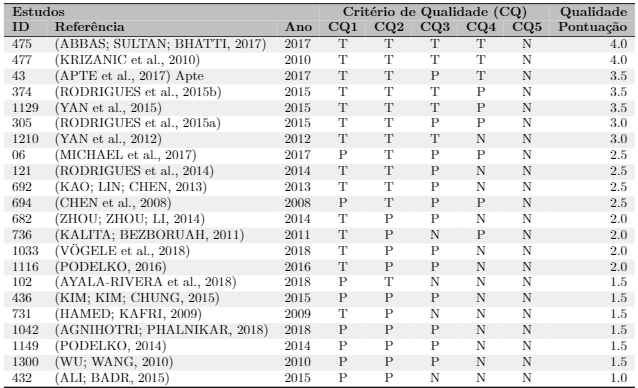
\includegraphics[width=0.90\textwidth]{Img/qualidade.PNG}
% \end{figure}
% \end{frame}

% \begin{frame}{{\sffamily  Revisão Sistemática: Ferramentas Citadas nos Estudos}}
% \begin{figure}
%     \centering
%     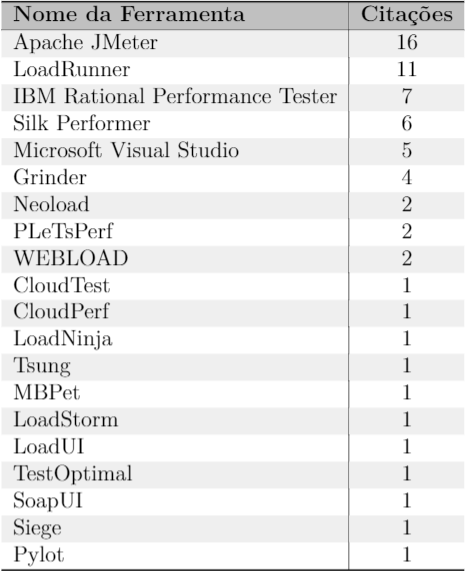
\includegraphics[width=0.45\textwidth]{Img/ferramentas.PNG}
% \end{figure}
% \end{frame}

% \begin{frame}{{\sffamily  Revisão Sistemática: Funcionalidades das Ferramentas}}
% \begin{figure}
%     \centering
%     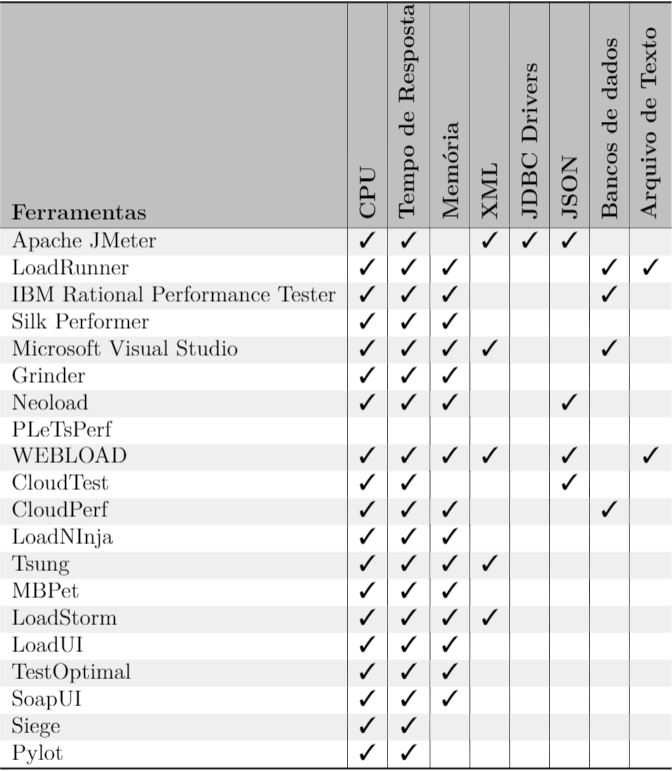
\includegraphics[width=0.52\textwidth]{Img/funcionalidades.PNG}
% \end{figure}
% \end{frame}

% \begin{frame}{{\sffamily  Revisão Sistemática: Formatos e Características do Relatório}}
% \begin{figure}
%     \centering
%     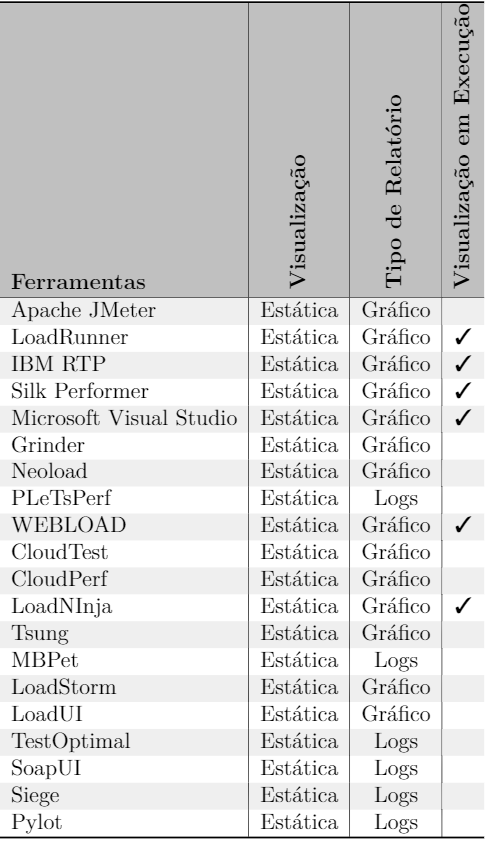
\includegraphics[width=0.35\textwidth]{Img/graficosferramentas.PNG}
% \end{figure}
% \end{frame}

% \begin{frame}{{\sffamily  Revisão Sistemática: Distribuição Geográfica dos Estudos}}
% \begin{figure}
%     \centering
%     \caption{Distribuição Geográfica dos Estudos} 
%     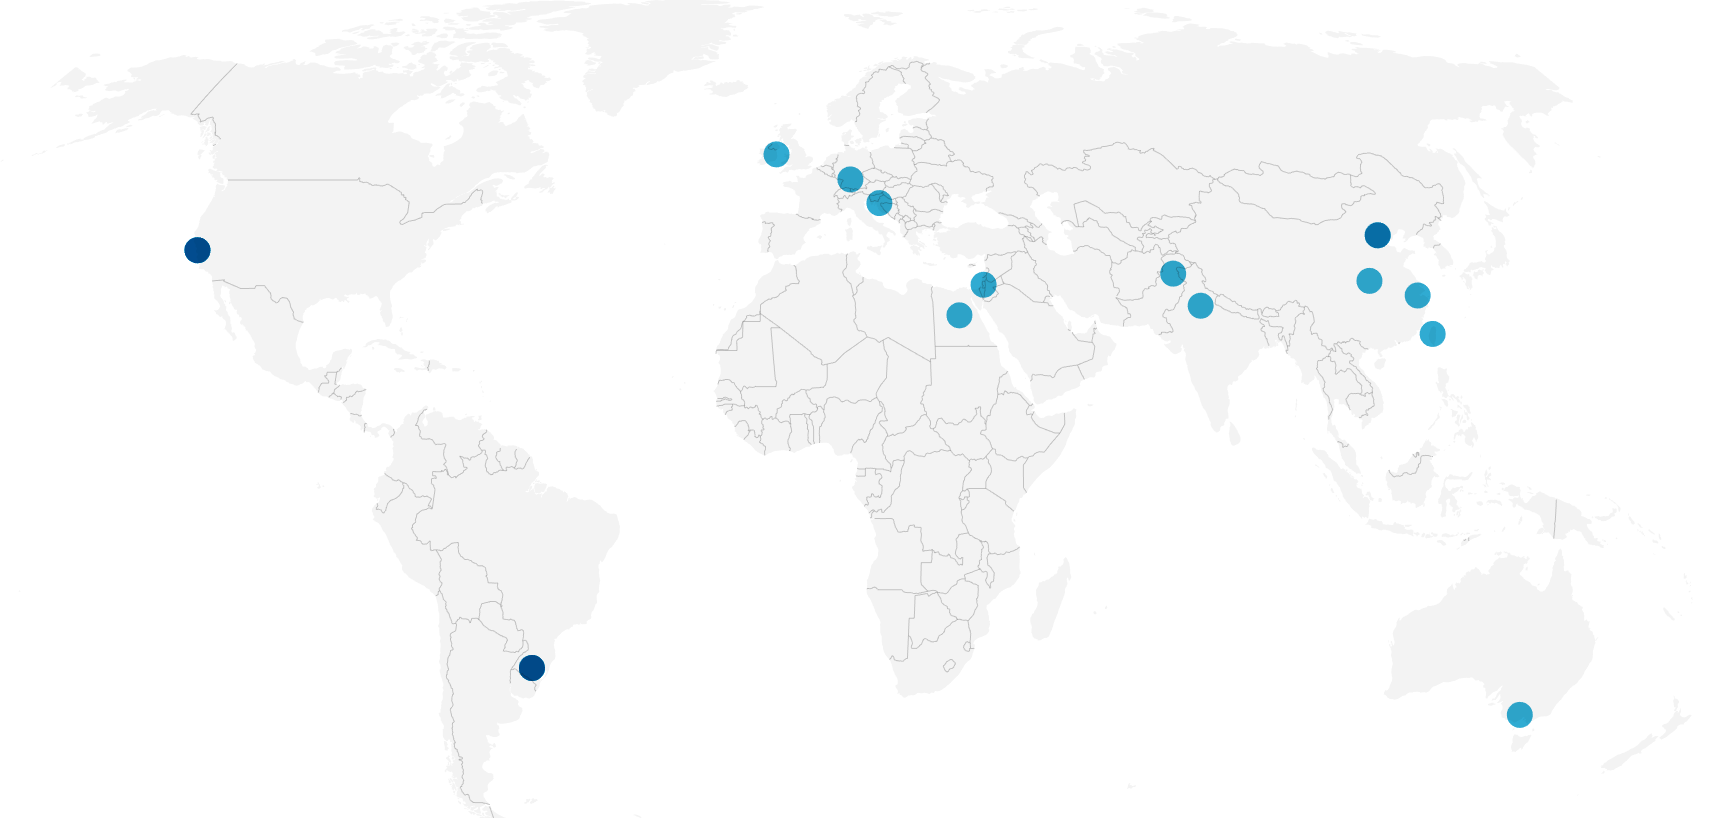
\includegraphics[width=0.95\textwidth]{Img/mapa.PNG}
% \end{figure}
% \end{frame}

% % \begin{frame}{{\sffamily  Revisão Sistemática: Anos de Publicação dos Estudos Selecionados.}}
% %     \begin{figure}
% %         \centering
% %         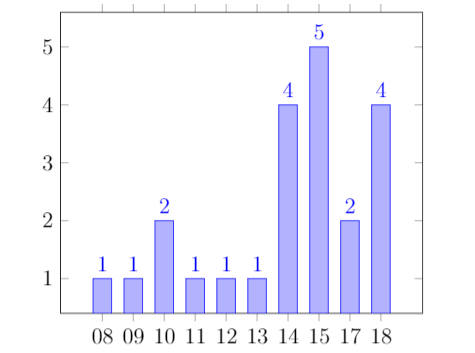
\includegraphics[width=0.70\textwidth]{Img/anosdepublicacao.PNG}
% %         \end{figure}
% % \end{frame}

% \begin{frame}{{\sffamily  Busca na Literatura Cinza: Motivação}}
%         \begin{block}{}
% 	\begin{itemize}%[<+->]
% 	    \item  Necessidade de encontrar ferramentas e bibliotecas de visualização de dados.
% 	    \item  \textit{Guidelines for including \textbf{Grey Literature} and conducting multivocal literature reviews in software engineering}. GAROUSI, V.
% 	    \end{itemize}
% \end{block}
% \end{frame}

% \begin{frame}{{\sffamily  Busca na Literatura Cinza: Ferramentas e Bibliotecas de Visualização de Dados}}
%     \begin{figure}
%         \centering
%         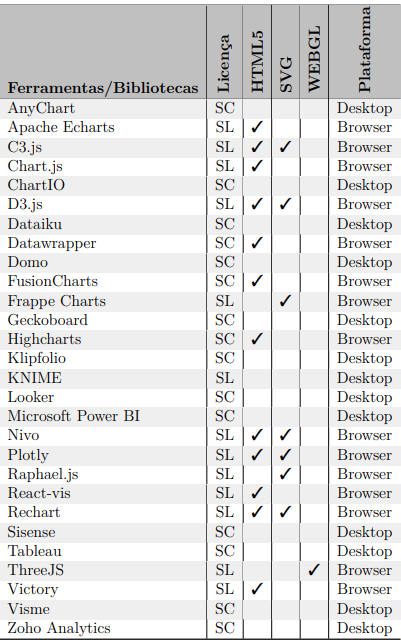
\includegraphics[width=0.33\textwidth]{Img/bibliotecas.png}
%         \end{figure}
% \end{frame}

% %######################################################################
% \section{Proposta}
% \subsection*{Proposta}
% %######################################################################


% \begin{frame}{{\sffamily  Requisitos}}
%     \begin{block}{}
% 	\begin{itemize}%[<+->]
% 	    \item  RQ1.A ferramenta precisa estar disponível sob licença open source.
% 	    \item  RQ2.A ferramenta tem de ser capaz de receber uma entrada de dados como parâmetro.
% 	    \item  RQ3.A ferramenta deve ser capaz de gerar gráficos a partir da entrada de dados.
% 	    \item  RQ4.A ferramenta deve ser capaz de apresentar dados de forma interativa.
% 	    \item  RQ5.A ferramenta deve automatizar a análise de resultados.
% 	\end{itemize}
% \end{block}
% \end{frame}

% \begin{frame}{{\sffamily Decisões de Projeto}}
%     \begin{block}{}
% 	\begin{itemize}%[<+->]
% 	    \item DP1. A ferramenta/biblioteca de visualização de dados deve ser \textit{open-source} (RQ1).
% 	    \item DP2. A ferramenta/biblioteca de visualização de dados deve ser capaz de receber uma entrada de dados (RQ2).
% 	    \item DP3. A ferramenta/biblioteca de visualização de dados tem de gerar gráficos a partir da entrada de dados (RQ3).
% 	\end{itemize}
% \end{block}
% \end{frame}

% \begin{frame}{{\sffamily Decisões de Projeto}}
%     \begin{block}{}
% 	\begin{itemize}%[<+->]
% 	    \item DP4. A ferramenta/biblioteca de visualização de dados deve possibilitar a apresentação de dados de forma interativa (RQ4).
% 	    \item DP5. A ferramenta deve fornecer alternativas para a análise de resultados automatizada (RQ5).
% 	\end{itemize}
% \end{block}
% \end{frame}

% \begin{frame}{{\sffamily  Arquitetura}}
%     \begin{figure}
%         \centering
%         \caption{Arquitetura da Proposta} 
%         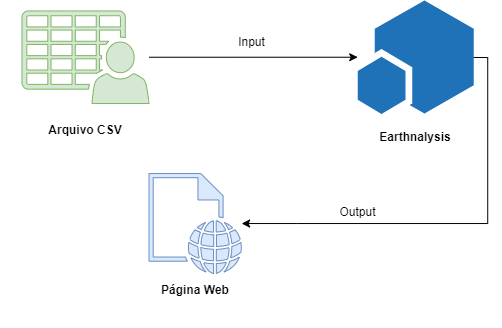
\includegraphics[width=0.85\textwidth]{Img/arquiteturaearth.png}
%         \end{figure}
% \end{frame}

% \begin{frame}{{\sffamily  Diagrama de Caso de Uso}}
%     \begin{figure}
%         \centering
%         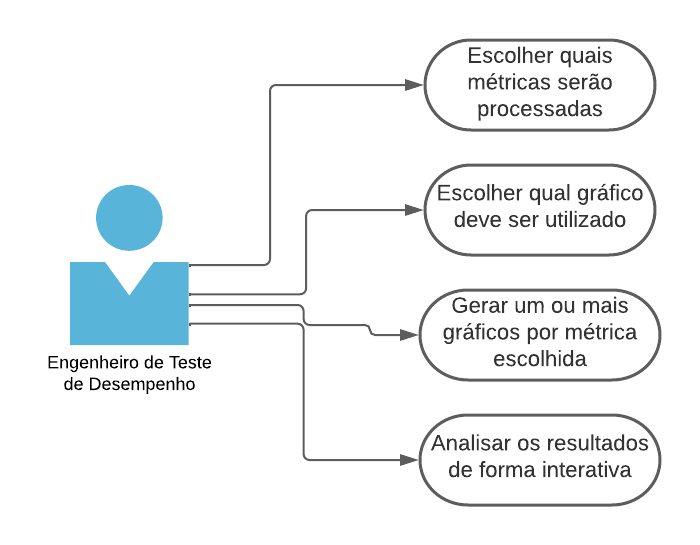
\includegraphics[width=0.75\textwidth]{Img/casodeuso.png}
%         \end{figure}
% \end{frame}

% \begin{frame}{{\sffamily  Caso de Uso 1. A ferramenta deve disponibilizar métricas \\para a análise dos resultados.}}
% \begin{figure}
%     \centering
%     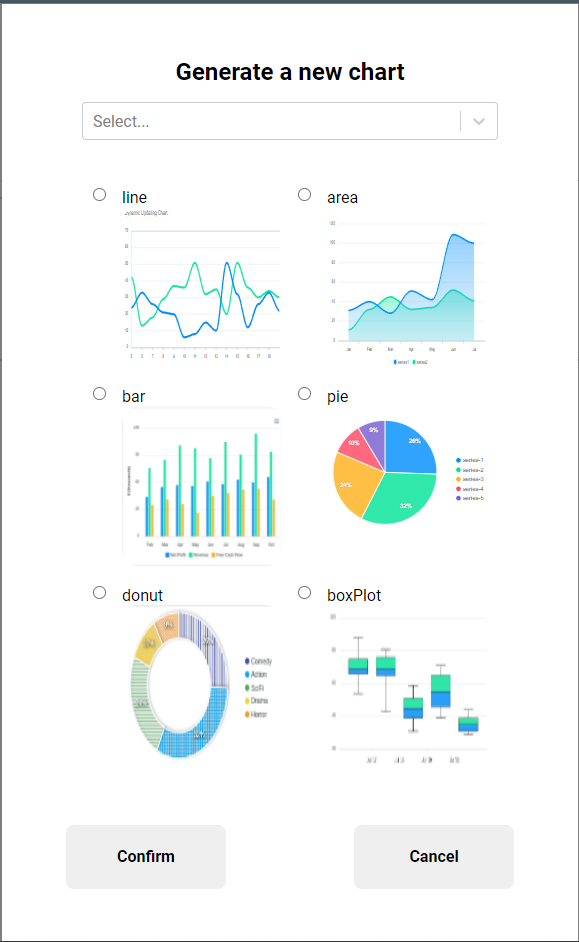
\includegraphics[width=0.33\textwidth]{Img/earthresultados.PNG}
% \end{figure}
% \end{frame}

% \begin{frame}{{\sffamily  Caso de Uso 2. A ferramenta deve ser capaz de gerar \\gráficos a partir da entrada de dados}}
% \begin{figure}
%     \centering
%     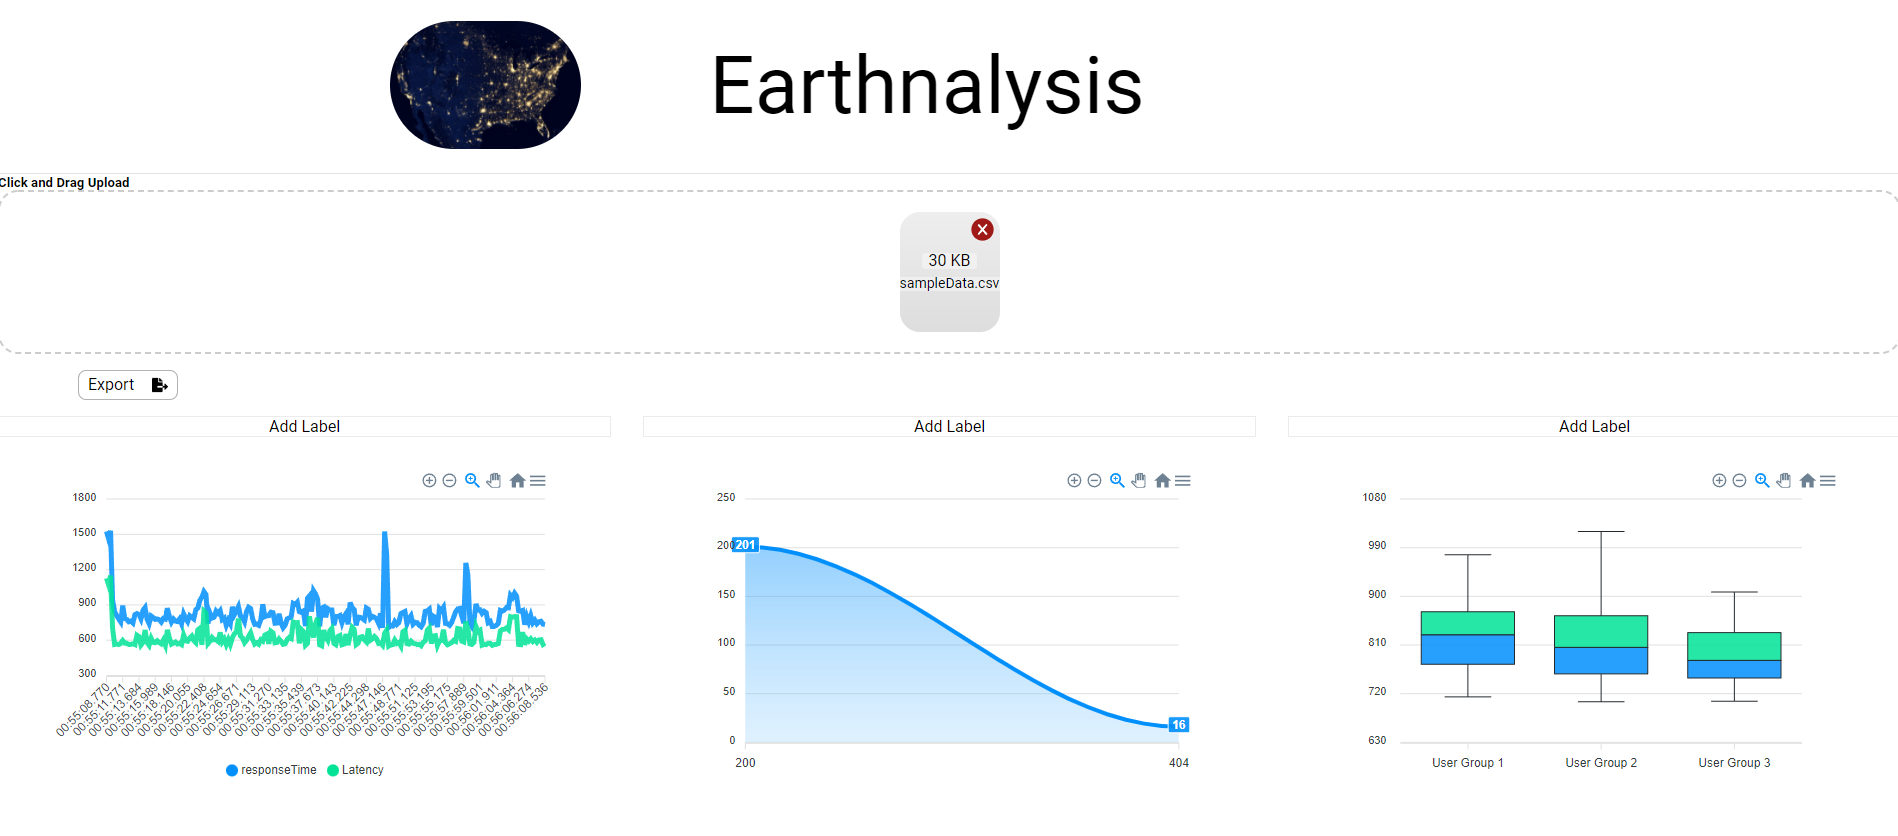
\includegraphics[width=0.95\textwidth]{Img/earthnalysis.png}
% \end{figure}
% \end{frame}

% %######################################################################
% \section{Avaliação}
% \subsection*{Mapeamento das Necessidades}

% %######################################################################

% \begin{frame}{{\sffamily  Mapeamento das Necessidades}}
%     \begin{block}{}
% 	\begin{itemize}%[<+->]
% 	    \item  Planejamento;
% 	    \SubItem{Estrutura estabelecida}
% 	    \SubItem{Estratégia das questões}
% 	    \item  Objetivo;
% 	    \SubItem{Entendimento das necessidades da indústria}
% 	    \SubItem{Coletar informações de profissionais da área}
% 	    \item  Execução.
% 	    \SubItem{Distribuição do questionário}
% 	    \SubItem{52 participantes, 8 países*}
% 	\end{itemize}
% \end{block}
% \end{frame}
% %######################################################################

% %######################################################################

% \begin{frame}{{\sffamily  Mapeamento das Necessidades - Perfil dos Respondentes}}
% \begin{block}{}
% \begin{figure}
%     \centering
%     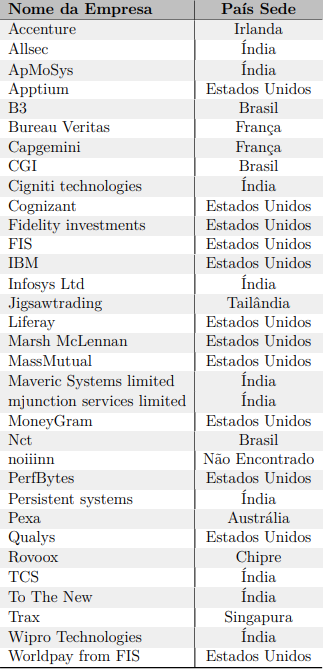
\includegraphics[width=0.25\textwidth]{Img/empresasmapeamento.png}
% \end{figure}
% \end{block}
% \end{frame}
% %######################################################################

% %######################################################################

% \begin{frame}{{\sffamily  Mapeamento das Necessidades - Nível Acadêmico}}
% \begin{block}{}
% \begin{figure}
%     \centering
%     \caption{Nível de formação acadêmica dos respondentes}
%     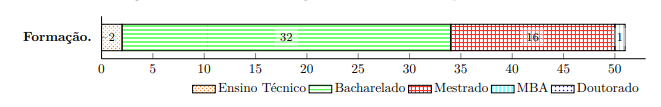
\includegraphics[width=0.85\textwidth]{Img/educacaomapeamento.png}
% \end{figure}
% \end{block}
% \end{frame}
% %######################################################################

% %######################################################################

% \begin{frame}{{\sffamily  Mapeamento das Necessidades - Nível de Experiência}}
% \begin{block}{}
%     \begin{figure}
%         \centering
%         \caption{Anos de Experiência na Indústria}
%         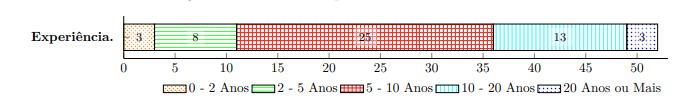
\includegraphics[width=0.85\textwidth]{Img/experienciamapeamento.png}
%     \end{figure}
%     \begin{figure}
%         \centering
%          \caption{Anos de Experiência como Engenheiro de Teste de Desempenho}
%         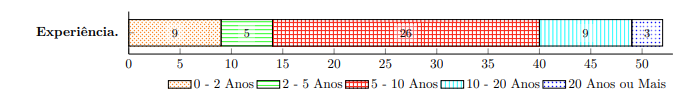
\includegraphics[width=0.85\textwidth]{Img/experienciatestermapeamento.png}
%     \end{figure}
% \end{block}
% \end{frame}
% %######################################################################

% %######################################################################

% \begin{frame}{{\sffamily  Mapeamento das Necessidades - Resultados}}
% \begin{block}{}
% 	\begin{itemize}%[<+->]
% 	    \item  Q1.\textit{How do you analyze the results of the performance test?} Do you use any tool? Which? (Como você analisa os resultados do teste de desempenho? Você usa alguma ferramenta? Qual?);
%             \SubItem{\textit{JMeter}, \textit{Dynatrace} e \textit{LoadRunner.}}
% 	    \item  Q2. \textit{What feature could help the process of analyzing the results?} (Que recurso poderia ajudar no processo de análise dos resultados?);
% 	        \SubItem{Gráficos, Comparação entre os testes executados, Customização, Visualização do tempo de resposta frente a outras métricas.}
% 	\end{itemize}
% \end{block}
% \end{frame}
% %######################################################################

% %######################################################################

% \begin{frame}{{\sffamily  Mapeamento das Necessidades - Questões Abertas}}
%     \begin{block}{}
% 	\begin{itemize}%[<+->]
% 	     \item  Q3. \textit{How do you rate the resources for analyzing results in performance testing tools?} (Como você classifica os recursos para análise de resultados em ferramentas de teste de desempenho?)
% 	     \item  Q4. \textit{How beneficial would be a solution that could be coupled with a performance test project, to have resources for the analysis of results?} (Quão benéfica seria uma solução que pudesse ser acoplada a um projeto de teste de desempenho, para ter recursos para a análise de resultados?)
% 	\end{itemize}
% \end{block}
% \end{frame}
% %######################################################################

% \begin{frame}{{\sffamily  Mapeamento das Necessidades - Questões Fechadas}}
% \begin{block}{}
% \begin{figure}
%     \centering
%     \caption{Classificação de 1 - 10 para pergunta \textbf{Q3.} e \textbf{Q4.}}
%     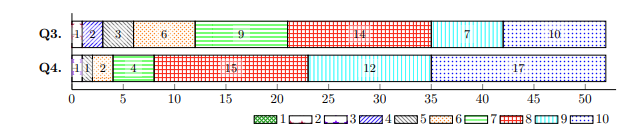
\includegraphics[width=0.95\textwidth]{Img/questoes.png}
% \end{figure}
% \end{block}
% \end{frame}
% %######################################################################

% \begin{frame}{{\sffamily  Mapeamento das Necessidades - Respostas}}
% \begin{block}{}
% 	\begin{itemize}%[<+->]
% 	    \item  Q5. \textit{Do you consider that generating graphs of the results is beneficial for the analysis of the results?} (Você considera que a geração de gráficos dos resultados é benéfica para a análise dos resultados?)
% 	\end{itemize}
% 	\begin{figure}
%         \centering
%         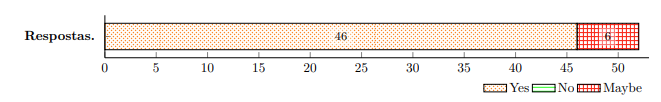
\includegraphics[width=0.95\textwidth]{Img/benefico.png}
%     \end{figure}
% \end{block}
% \end{frame}
% %######################################################################

% %######################################################################
% %\section{Avaliação}
% \subsection*{Avaliação Exploratória}

% %######################################################################

% \begin{frame}{{\sffamily Avaliação Exploratória}}
%     \begin{block}{}
% 	\begin{itemize}%[<+->]
% 	    \item  Planejamento;
% 	    \SubItem{Estrutura estabelecida}
% 	    \SubItem{Estratégia das questões}
% 	    \item  Objetivo;
% 	    \SubItem{Entendimento das necessidades da indústria}
% 	    \SubItem{Coletar informações de profissionais da área}
% 	    \item  Execução.
% 	    \SubItem{Distribuição do questionário}
% 	    \SubItem{15 participantes, 5 países*}
% 	\end{itemize}
% \end{block}
% \end{frame}
% %######################################################################

% %######################################################################

% \begin{frame}{{\sffamily Avaliação Exploratória - Perfil dos Respondentes}}
% \begin{block}{}
% \begin{figure}
%     \centering
%     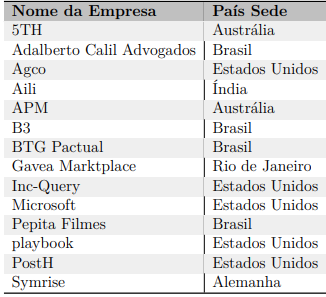
\includegraphics[width=0.60\textwidth]{Img/empresasavaliacao.png}
% \end{figure}
% \end{block}
% \end{frame}
% %######################################################################

% \begin{frame}{{\sffamily  Avaliação Exploratória - Nível acadêmico}}
% \begin{block}{}
% \begin{figure}
%     \centering
%     \caption{Nível de formação acadêmica dos respondentes}
%     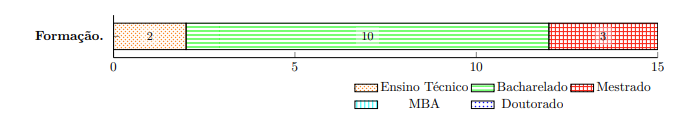
\includegraphics[width=0.85\textwidth]{Img/educacaoavaliacao.png}
% \end{figure}
% \end{block}
% \end{frame}
% %######################################################################

% \begin{frame}{{\sffamily  Avaliação Exploratória - Nível de Experiência}}
% \begin{block}{}
%     \begin{figure}
%         \centering
%         \caption{Anos de Experiência na Indústria}
%         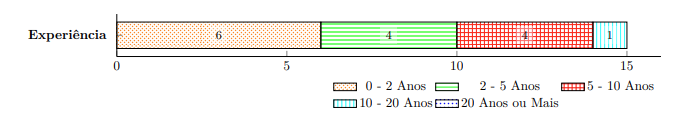
\includegraphics[width=0.85\textwidth]{Img/experienciaavaliacao.png}
%     \end{figure}
%     \begin{figure}
%         \centering
%         \caption{Anos de Experiência como Engenheiro de Teste de Desempenho}
%         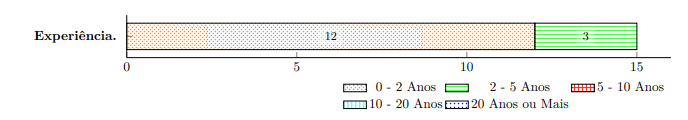
\includegraphics[width=0.85\textwidth]{Img/experienciatesteravaliacao.png}
%   \end{figure}
% \end{block}
% \end{frame}
% %######################################################################

% \begin{frame}{{\sffamily Avaliação Exploratória - Avaliação Técnica}}
%     \begin{block}{}
% 	\begin{itemize}%[<+->]
% 	    \item \textbf{QF1.} \textit{The tool help in analyzing performance test results.} (A ferramenta ajuda na análise dos resultados dos testes de desempenho.)
%         \item \textbf{QF2.} \textit{I would recommend this tool to a friend.} (Eu recomendaria esta ferramenta a um amigo.)
%         \item \textbf{QF3.} \textit{Using the tool can reduce the time spent analyzing the performance test results?} (O uso da ferramenta pode reduzir o tempo gasto analisando os resultados dos testes de desempenho?)
% 	\end{itemize}
% \end{block}
% \end{frame}
% %######################################################################

% \begin{frame}{{\sffamily Avaliação Exploratória - Avaliação Técnica}}
%     \begin{block}{}
% 	\begin{itemize}%[<+->]
%         \item \textbf{QF4.} \textit{Earthnalysis produce the expected graphs for the analysis of performance testing results.} (Earthnalysis produz os gráficos esperados para a análise dos resultados dos testes de desempenho.)
%         \item \textbf{QF5.} \textit{Using the tool can improve my performance when analyzing results of performance tests.} (O uso da ferramenta pode melhorar meu desempenho ao analisar resultados de testes de desempenho.)
%         \item \textbf{QF6.} \textit{The tool is fast in generating graphics and processing .CSV.} (A ferramenta é rápida na geração de gráficos e no processamento de .CSV.)
% 	\end{itemize}
% \end{block}
% \end{frame}
% %######################################################################

% \begin{frame}{{\sffamily  Avaliação Exploratória - Respostas}}
% \begin{block}{}
%     \begin{figure}
%         \centering
%         \caption{Respostas da Avaliação Técnica}
%         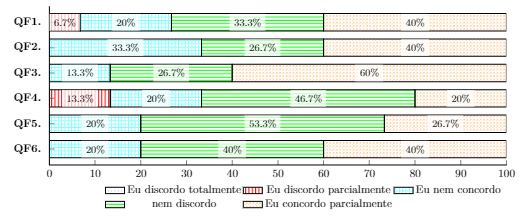
\includegraphics[width=0.85\textwidth]{Img/avaliacaotecnica.PNG}
%     \end{figure}
% \end{block}
% \end{frame}
% %######################################################################


% \begin{frame}{{\sffamily Avaliação Exploratória - Avaliação de Usabilidade}}
%     \begin{block}{}
% 	\begin{itemize}%[<+->]
%         \item \textbf{QU1.} \textit{Earthnalysis was easy to use.} (Earthnalysis foi fácil de usar.)
%         \item \textbf{QU2.} \textit{Earthnalysis is a good idea.} (Earthnalysis é uma boa ideia.)
%         \item \textbf{QU3.} \textit{I liked using Earthnalysis.} (Eu gostei de usar a Earthnalysis.)
%         \item \textbf{QU4.} \textit{Earthnalysis can facilitate the analysis of performance test results.} (Earthnalysis pode facilitar a análise dos resultados dos testes de desempenho.)
% 	\end{itemize}
% \end{block}
% \end{frame}
% %######################################################################

% \begin{frame}{{\sffamily  Avaliação Exploratória - Respostas}}
% \begin{block}{}
%     \begin{figure}
%         \centering
%         \caption{Respostas da Avaliação de Usabilidade}
%         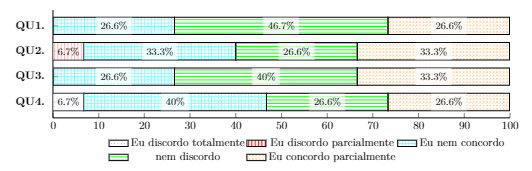
\includegraphics[width=0.95\textwidth]{Img/avaliacaodeusabilidade.PNG}
%     \end{figure}
% \end{block}
% \end{frame}
% %######################################################################

% \begin{frame}{{\sffamily  valiação Exploratória - Questões Abertas}}
%     \begin{block}{}
% 	\begin{itemize}%[<+->]
% 	     \item \textbf{QA1.} \textit {What were the positive points in your experience with the tool?} (Quais foram os pontos positivos em sua experiência com a ferramenta?)
% 	        \SubItem{Facilidade de Uso, Intuitiva, Rápida geração de gráficos.}
% 	     \item \textbf{QA2.} \textit {What were the negative points in your experience with the tool?} (Quais foram os pontos negativos em sua experiência com a ferramenta?)
% 	        \SubItem{Interface muito simples, apenas um formato aceito como entrada de dados.}
% 	\end{itemize}
% \end{block}
% \end{frame}
% %######################################################################

% \begin{frame}{{\sffamily Avaliação Exploratória - Avaliação de Afeição}}
%     \begin{block}{}
% 	\begin{itemize}%[<+->]
% 	    \item \textit{Modelo do Circumplexo de Russell} 
%         \item \textbf{QR1.} \textit {Mood while performing the evaluation.} (Humor ao realizar a avaliação.)
%         \item \textbf{QR2.} \textit {Mood while using the tool.} (Humor ao usar a ferramenta.)
% 	\end{itemize}
% \end{block}
% \end{frame}
% %######################################################################

% %######################################################################

% \begin{frame}{{\sffamily  Avaliação Exploratória - Níveis de Afeição }}
% \begin{block}{}
%   \begin{figure}
%         \centering
%         \caption{Opções disponíveis para responder a QR1 e QR2.}
%         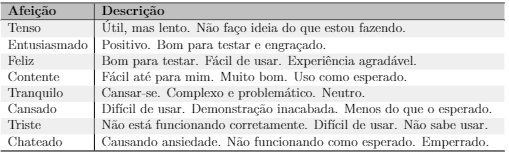
\includegraphics[width=0.99\textwidth]{Img/afeicao.PNG}
%     \end{figure}
% \end{block}
% \end{frame}
% %######################################################################

% %######################################################################

% \begin{frame}{{\sffamily  Avaliação Exploratória - Respostas}}
% \begin{block}{}
%   \begin{figure}
%         \centering
%         \caption{Humor enquanto executou a avaliação} 
%         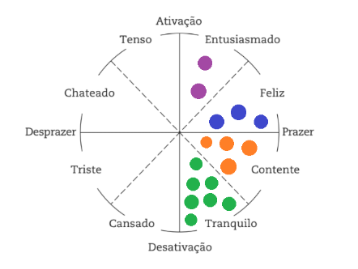
\includegraphics[width=0.60\textwidth]{Img/russell.PNG}
%     \end{figure}
% \end{block}
% \end{frame}
% %######################################################################

% %######################################################################

% \begin{frame}{{\sffamily  Avaliação Exploratória - Respostas}}
% \begin{block}{}
% \begin{figure}
%     \centering
%     \caption{Humor enquanto utilizou a ferramenta} 
%     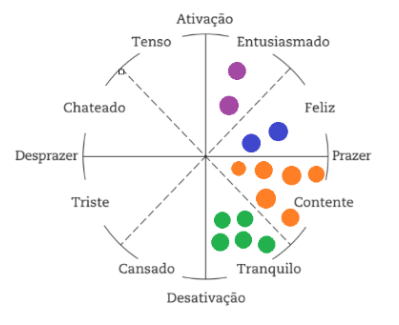
\includegraphics[width=0.55\textwidth]{Img/russell2.PNG}
% \end{figure}
% \end{block}
% \end{frame}
% %######################################################################

% \begin{frame}{{\sffamily Avaliação Exploratória - Ameaças à Validade do Estudo}}
%     \begin{block}{}
% 	\begin{itemize}%[<+->]
% 	    \item Validade do Constructo:
% 	        \SubItem{Criação de perguntas embasadas nos trabalhos relacionados.}
%         \item Validade Interna:
%             \SubItem{Estratégias para reduzir cansaço e desmotivação.}
%         \item Validade Externa:
%             \SubItem{Amostra representativa.}
%         \item Validade de Conclusão:
%             \SubItem{Estratégias para não ter um público enviesado.}
% 	\end{itemize}
% \end{block}
% \end{frame}
% %######################################################################


% %######################################################################
% \section{Considerações Finais}
% \subsection*{Considerações Finais}

% %######################################################################

% \begin{frame}{{\sffamily  Atividades Desenvolvidas}}
%     \begin{block}{}
% 	\begin{itemize}%[<+->]
% 	    \item  Levantamento do estado da arte;
% 	    \item  Elaboração da proposta;
% 	    \item  Desenvolvimento da ferramenta;
% 	    \item  Avaliação da ferramenta.
% 	\end{itemize}
% \end{block}
% \end{frame}

% %######################################################################

% \subsection*{Considerações Finais}

% %######################################################################

% \begin{frame}{{\sffamily  Lições Aprendidas e Relatos de Experiência}}
%     \begin{block}{}
% 	\begin{itemize}%[<+->]
% 	    \item Dificuldades encontradas;
% 	    \item Teste de desempenho na indústria;
% 	    \item Adesão na utilização da ferramenta desenvolvida.
% 	\end{itemize}
% \end{block}
% \end{frame}

% %######################################################################

% \begin{frame}{{\sffamily Earthnalysis - Uma Proposta de Visualização de Dados \\a partir de Relatórios de Teste de Desempenho}}
% \begin{block}{\begin{center}\huge{Perguntas?}\end{center}}
% 	\begin{center}
% 		\huge{}
% 	\end{center}
% \end{block}
% \begin{block}{Sobre:}
% 	\begin{itemize}%[<+->]
% 	    \item \href{http://lesse.com.br/}{{\color{blue}lesse.com.br}}
% 	    \item \href{http://novoportal.unipampa.edu.br/novoportal/}{{\color{blue}unipampa.edu.br}}
%     \end{itemize}
% \end{block}
% \end{frame}

% %######################################################################

\begin{frame}[plain,t]
	\titlepage
\end{frame}

\end{document}